\chapter{Android App}
\label{ch:app}
Kern dieser Projektarbeit ist die Android App, die als Benutzeroberfläche der digitalen Kaffeekasse dient.
Sie basiert auf Grundlagen, welche durch Android Jetpack gelegt wurden.
In diesem Kapitel werden Funktionalität, Architektur, verwendete Android Jetpack Komponenten und Bibliotheken sowie Konfiguration der App vorgestellt.

\section{Funktionalität}
\label{sec:app:functionality}
Beim erstmaligen Starten der App werden Nutzer gebeten ihren Account auszuwählen.
Alternativ können sie den Modus für eine geteilte Verwendung starten, welcher am Ende diese Abschnittes erläutert wird.
Der zugehörige Dialog ist in \autoref{fig:app:functionality:selection:dialog} zu sehen.
\begin{figure}%
	\centering
	\subfloat{{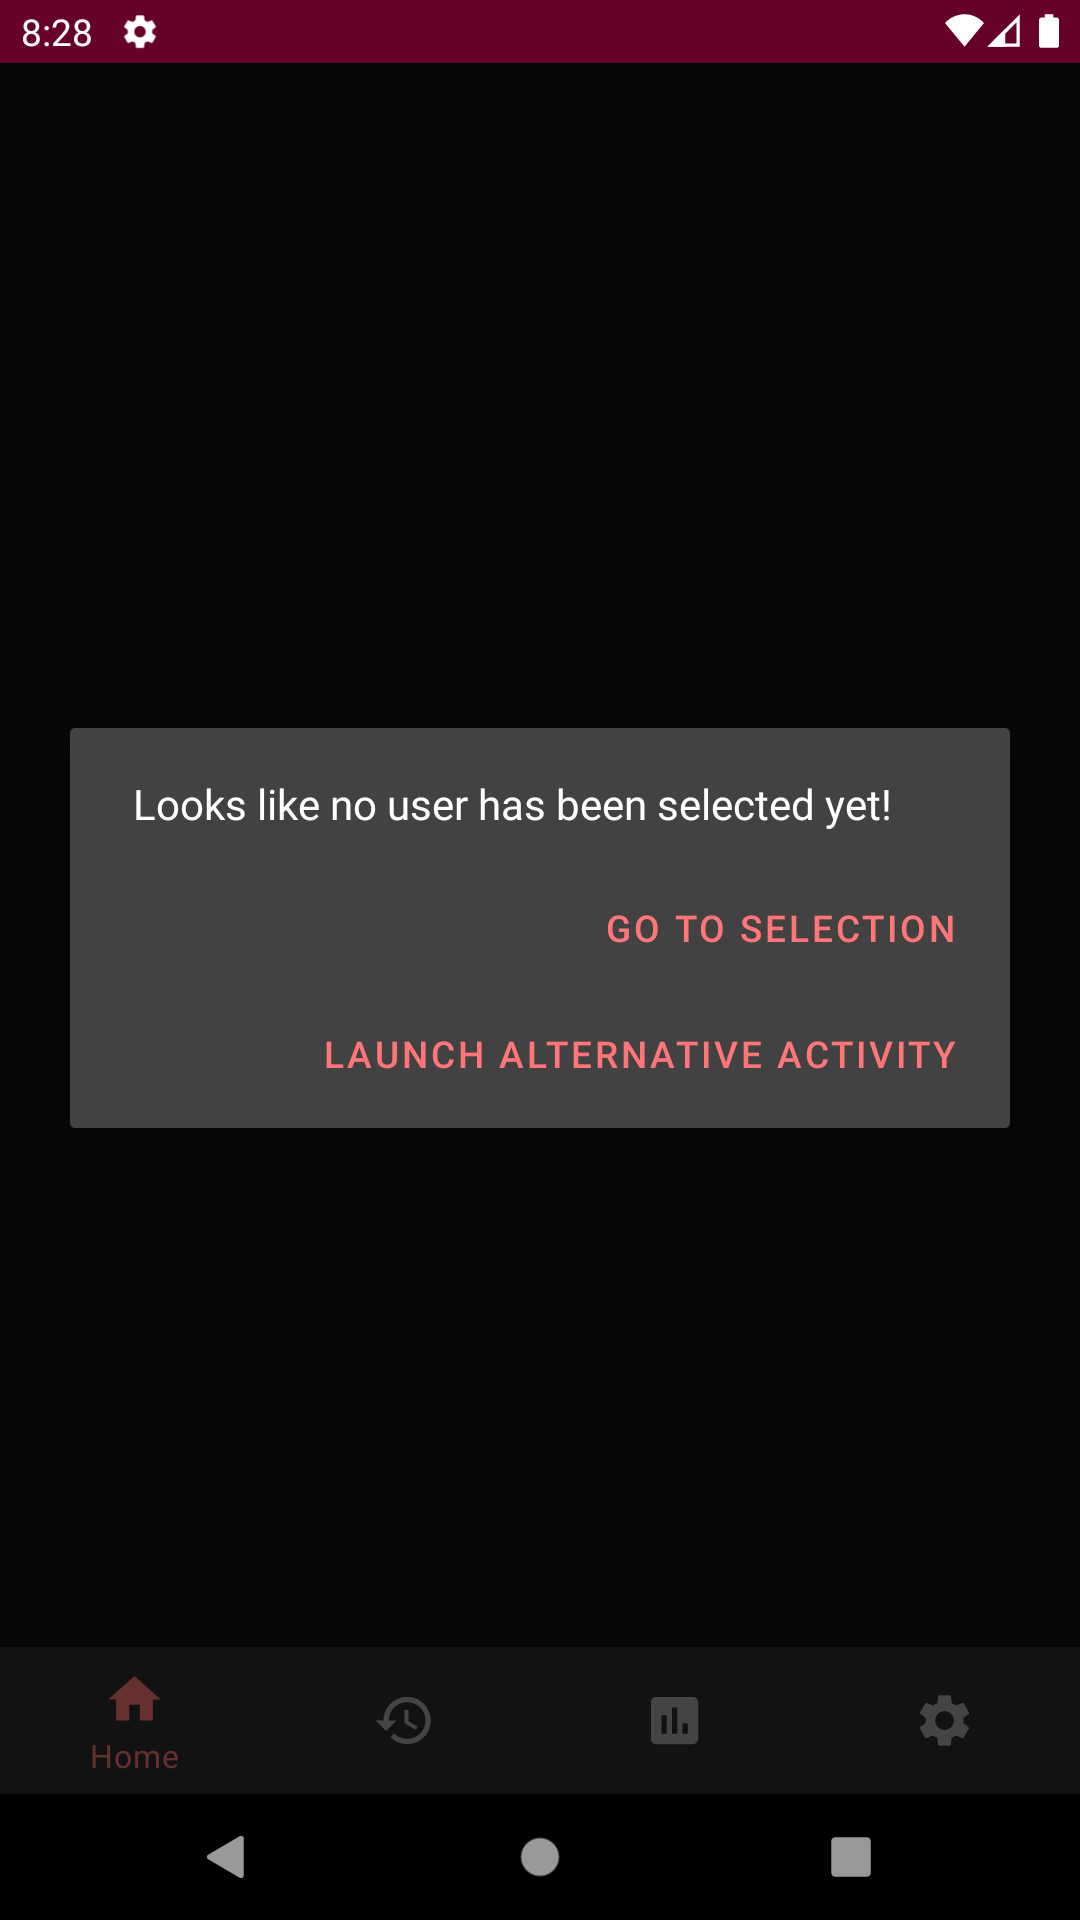
\includegraphics[height=8cm,keepaspectratio]{./img/screenshots/greetings-dialog.png}\label{fig:app:functionality:selection:dialog}}}%
	\qquad
	\subfloat{{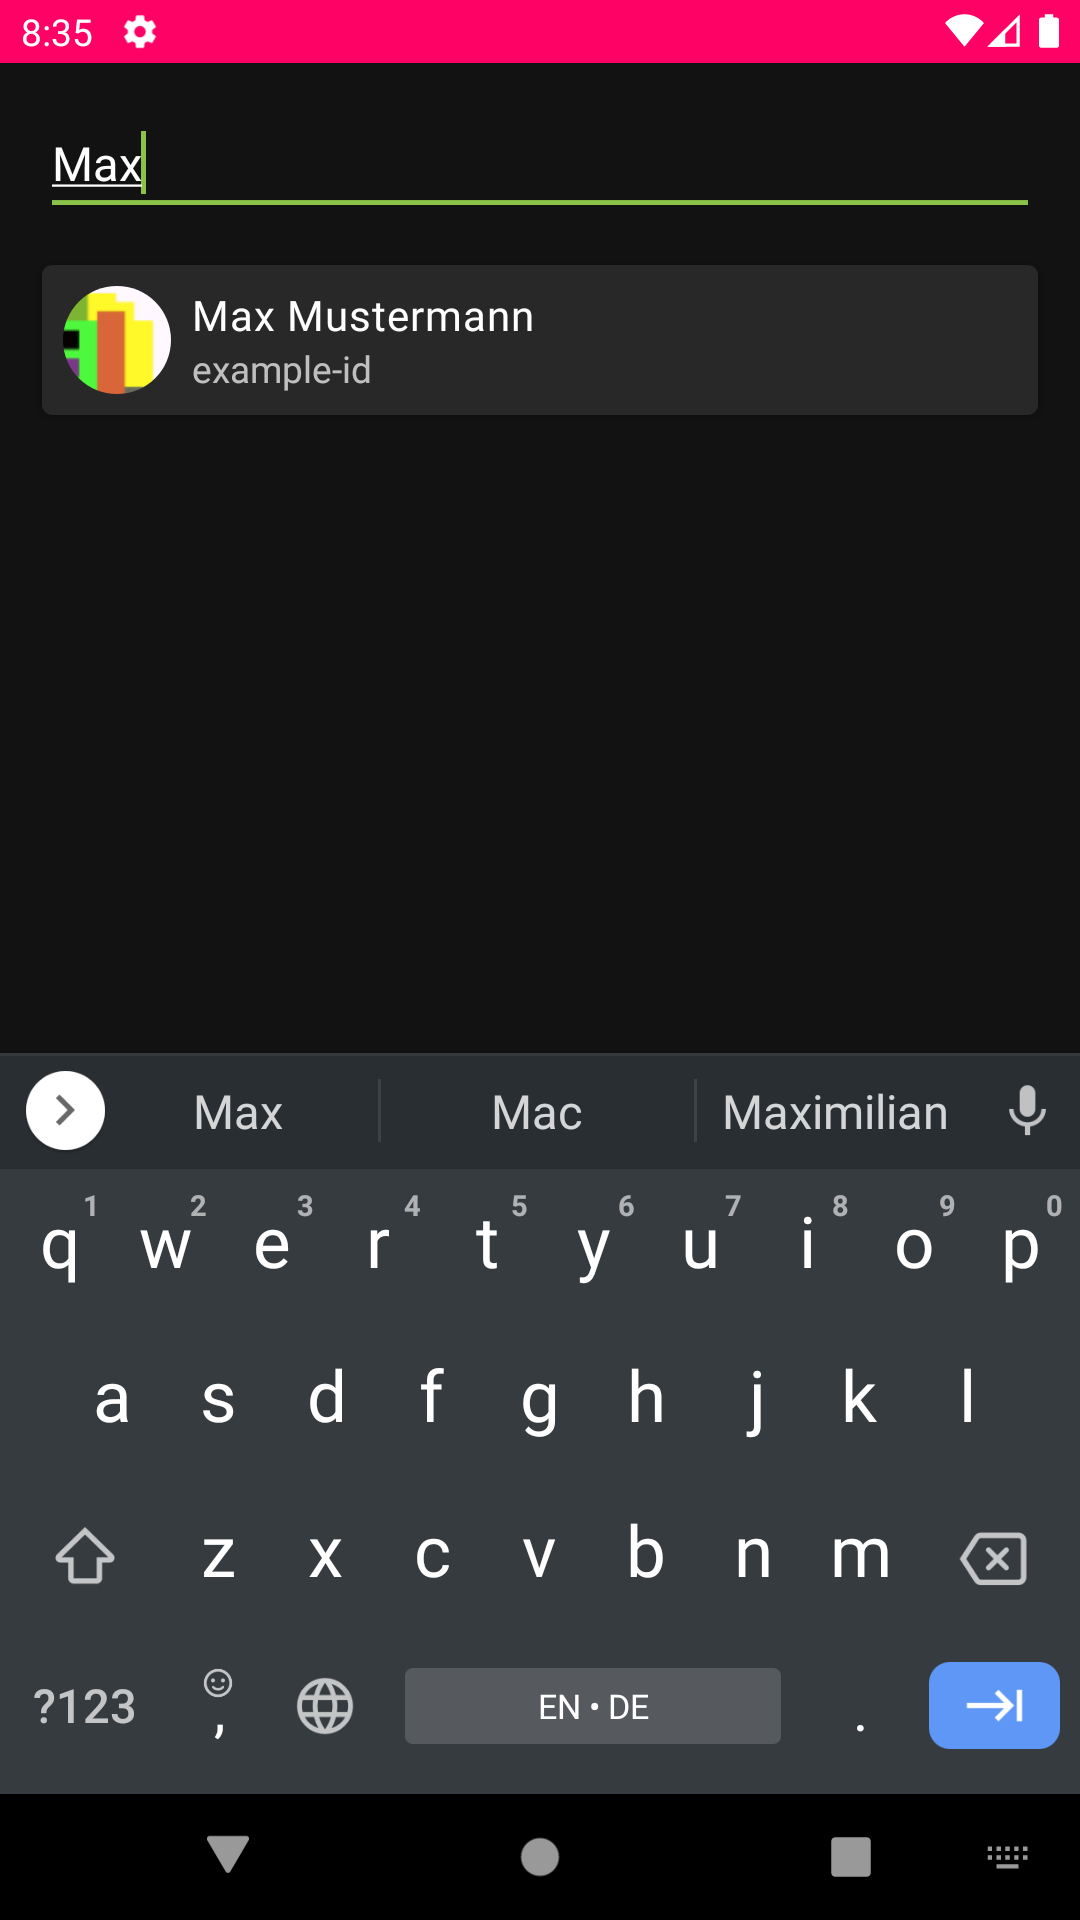
\includegraphics[height=8cm,keepaspectratio]{./img/screenshots/user-search.png}\label{fig:app:functionality:selection:search}}}%
	\caption{Begrüßungsdialog und Nutzerauswahl}%
	\label{fig:app:functionality:selection}%
\end{figure}

Die Nutzerauswahl zeigt eine Liste aller existierenden Nutzer an und ermöglicht es diese Interaktiv zu filtern.
Suchergebnisse werden unmittelbar angezeigt und benötigen keine zusätzlichen Eingaben (siehe \autoref{fig:app:functionality:selection:search}).
Nachdem ein Nutzer durch Klicken ausgewählt wurde, öffnet sich die Hauptseite der App.
Dort werden Informationen des ausgewählten Nutzers und verfügbare Artikel angezeigt.
Auch diese lassen sich analog zu Nutzern filtern und durch klicken auswählen, wie in \autoref{fig:app:functionality:home:search} sichtbar.
Falls eine stornierbare Transaktion vorliegt wird diese ebenfalls hier angezeigt (siehe \autoref{fig:app:functionality:home:transaction}).
Durch Klicken auf das Profilbild, beziehungsweise dessen Platzhalter, kann dieses bearbeitet oder entfernt werden.
\begin{figure}%
	\centering
	\subfloat{{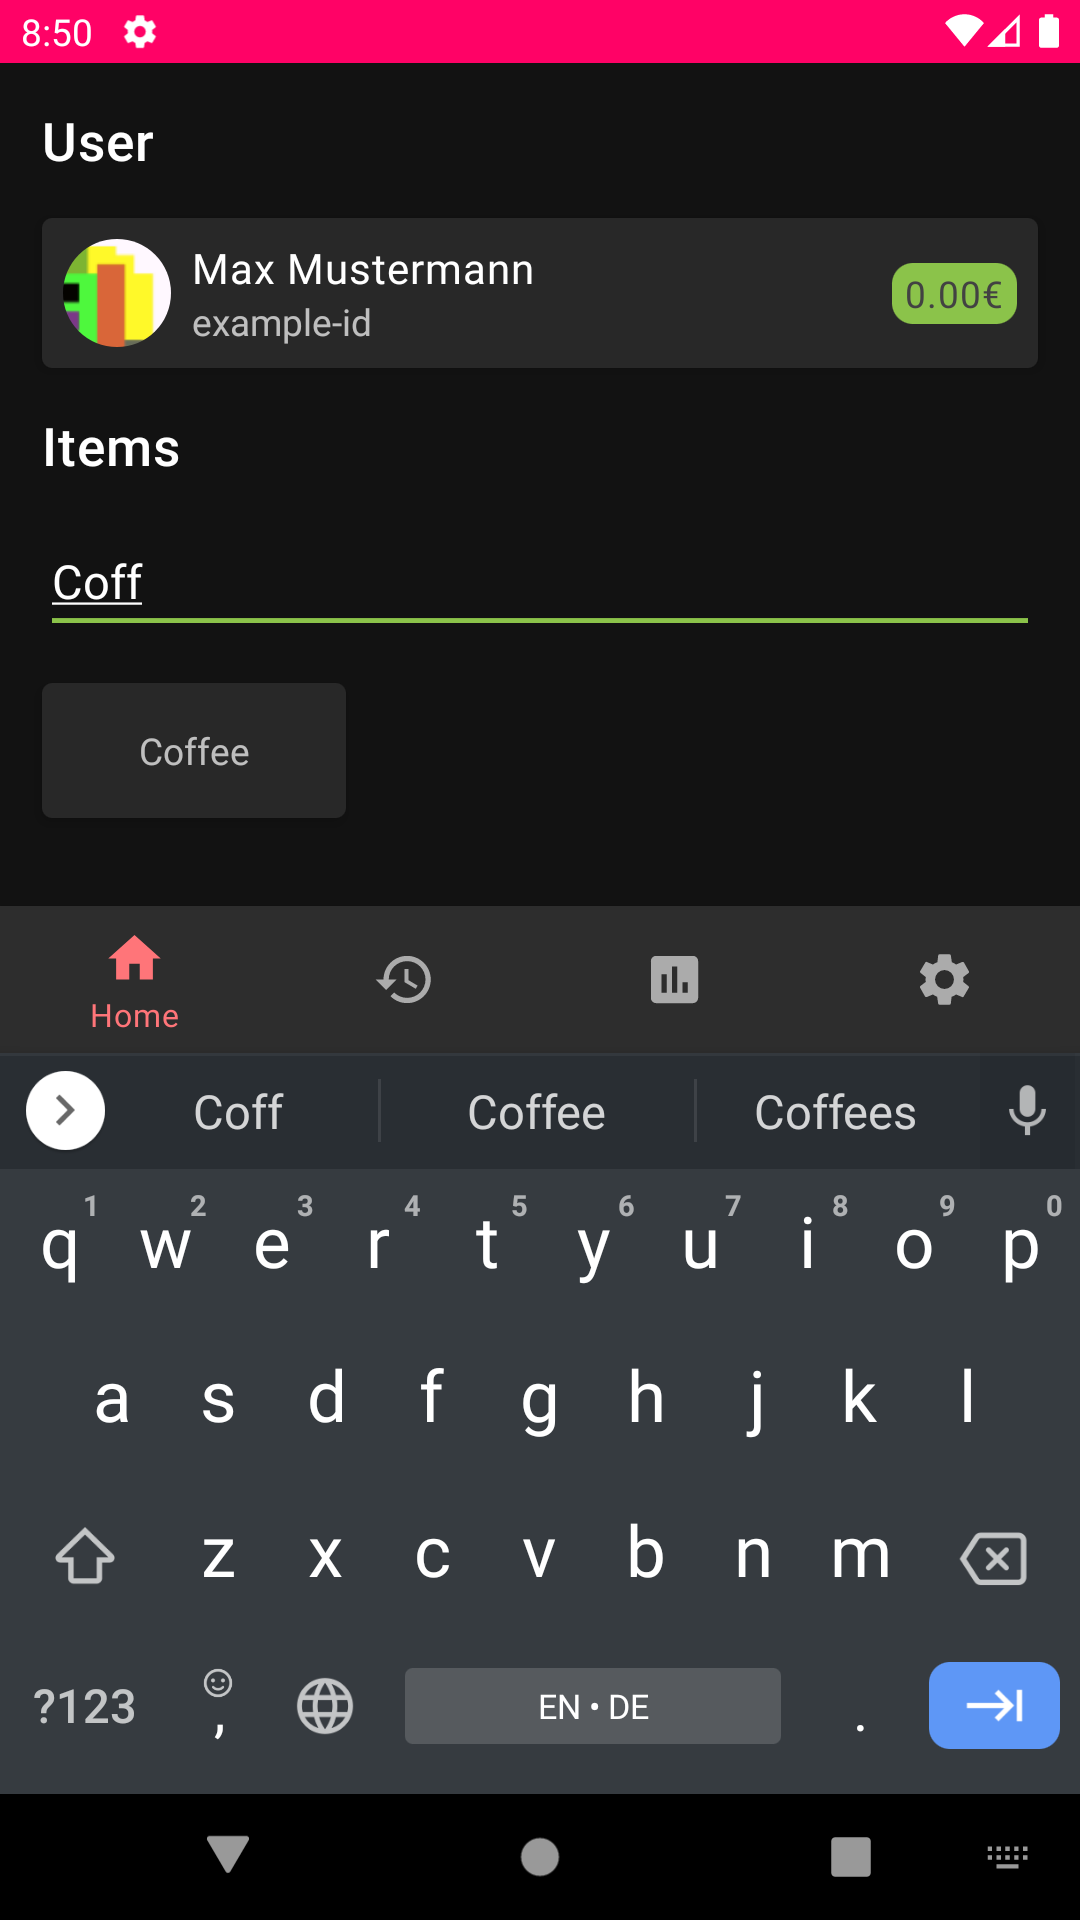
\includegraphics[height=8cm,keepaspectratio]{./img/screenshots/home-fragment.png}\label{fig:app:functionality:home:search}}}%
	\qquad
	\subfloat{{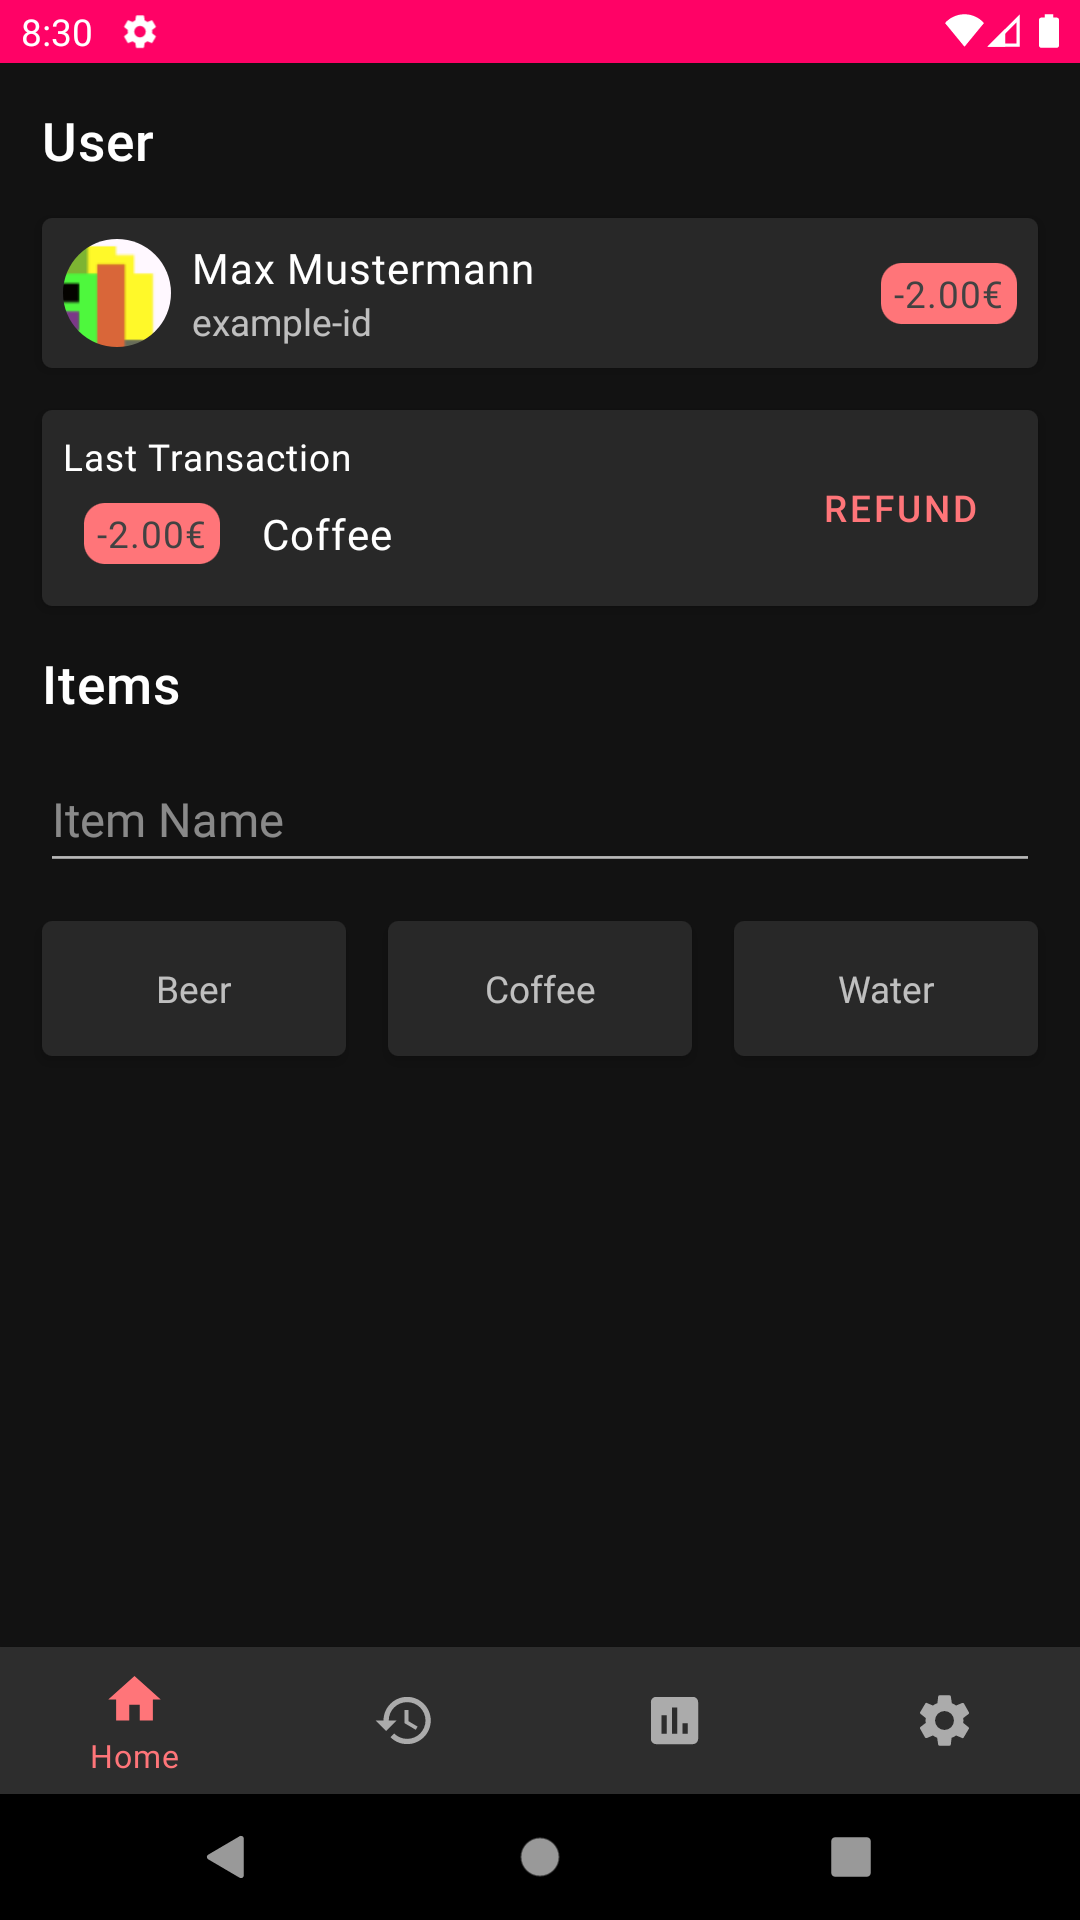
\includegraphics[height=8cm,keepaspectratio]{./img/screenshots/home-fragment-transaction.png}\label{fig:app:functionality:home:transaction}}}%
	\caption{Hauptseite}%
	\label{fig:app:functionality:home}%
\end{figure}

Die Artikelseite zeigt neben Preis und Name des Artikels auch alle Transaktionen des aktiven Nutzers an, die zu einem Artikel gehören.
Falls es sich um einen Artikel mit begrenztem Bestand handelt, wird auch dieser angezeigt und bei Transaktionen aktualisiert.
Zudem können Stornierungen auch von der Seite des betroffenen Artikels durchgeführt werden, wie in \autoref{fig:app:functionality:item} zu sehen ist.
Wie auch bei der Hauptseite, ist die Option nur während des gültigen Zeitrahmens von 60 Sekunden verfügbar und verschwindet selbstständig nach Ablaufen der Zeit.
\begin{figure}%
	\centering
	\subfloat{{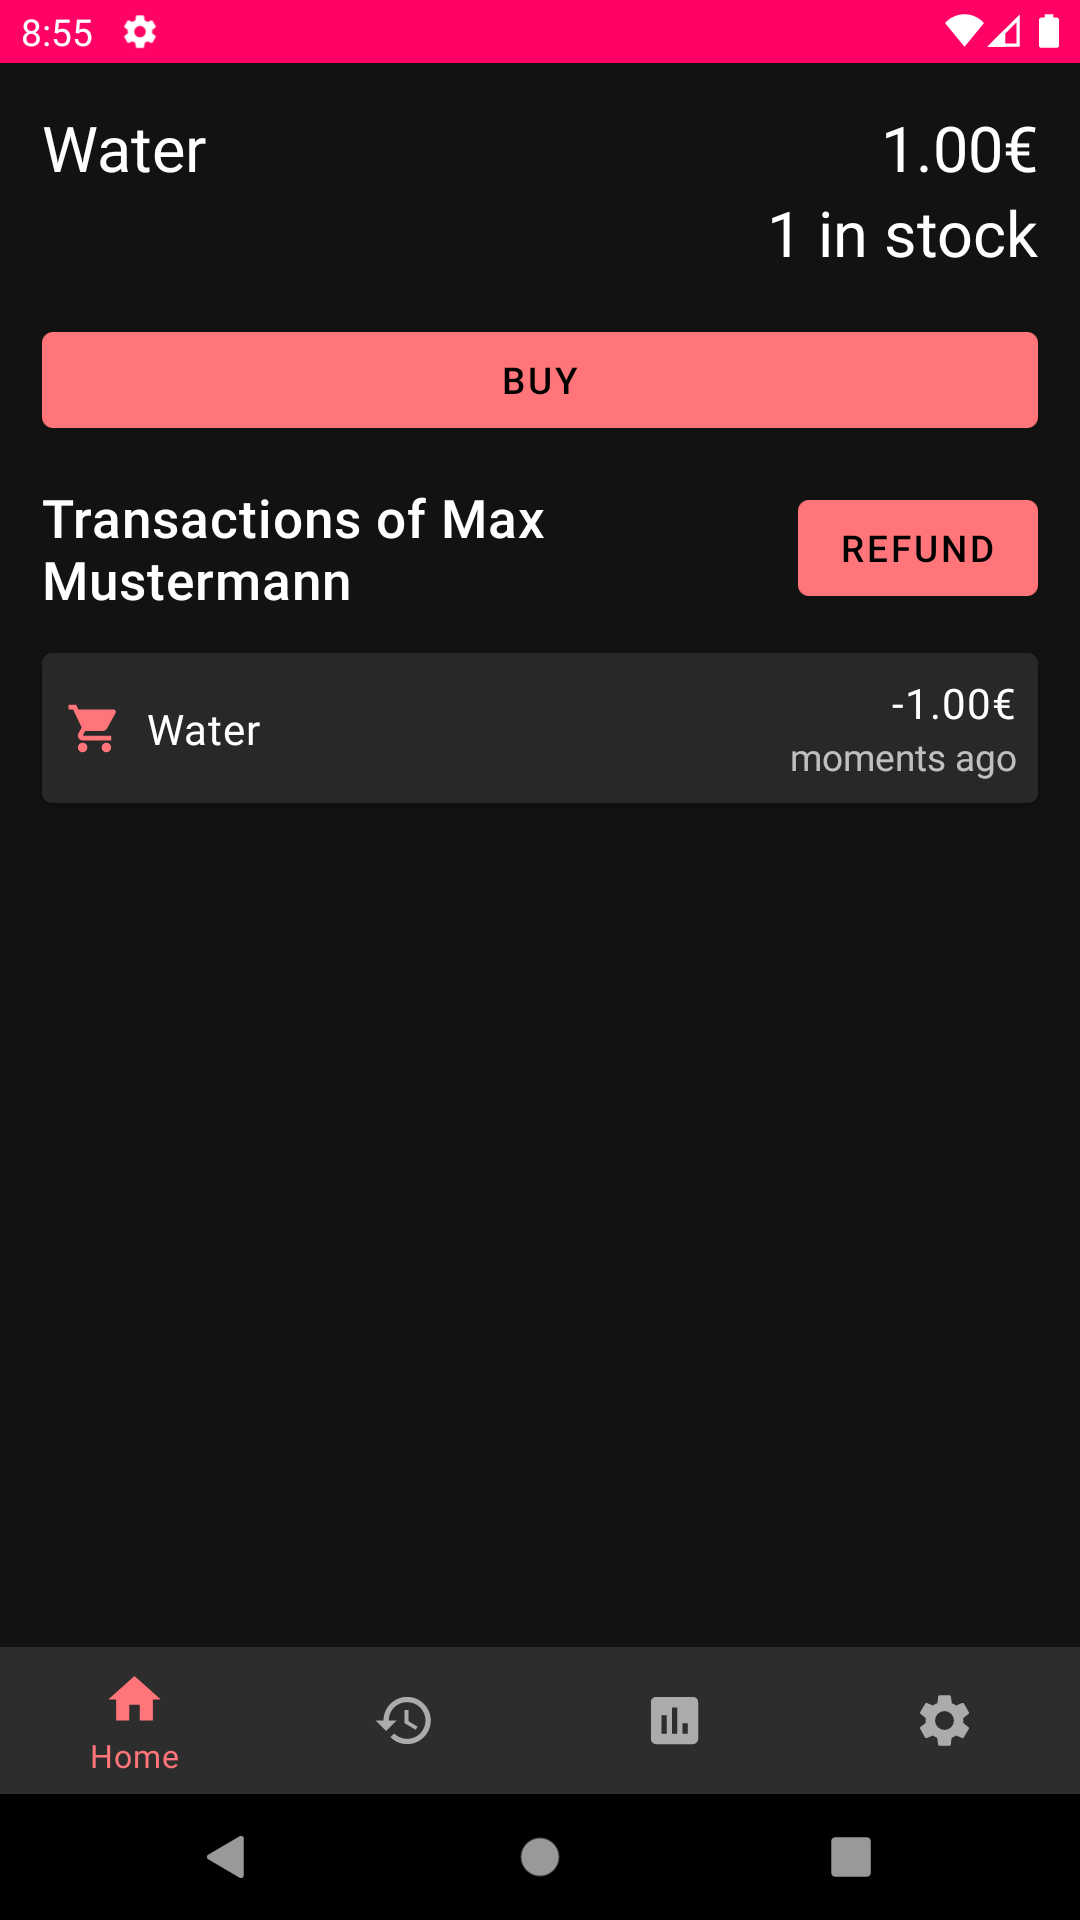
\includegraphics[height=8cm,keepaspectratio]{./img/screenshots/item-purchased.png}\label{fig:app:functionality:item:purchase}}}%
	\qquad
	\subfloat{{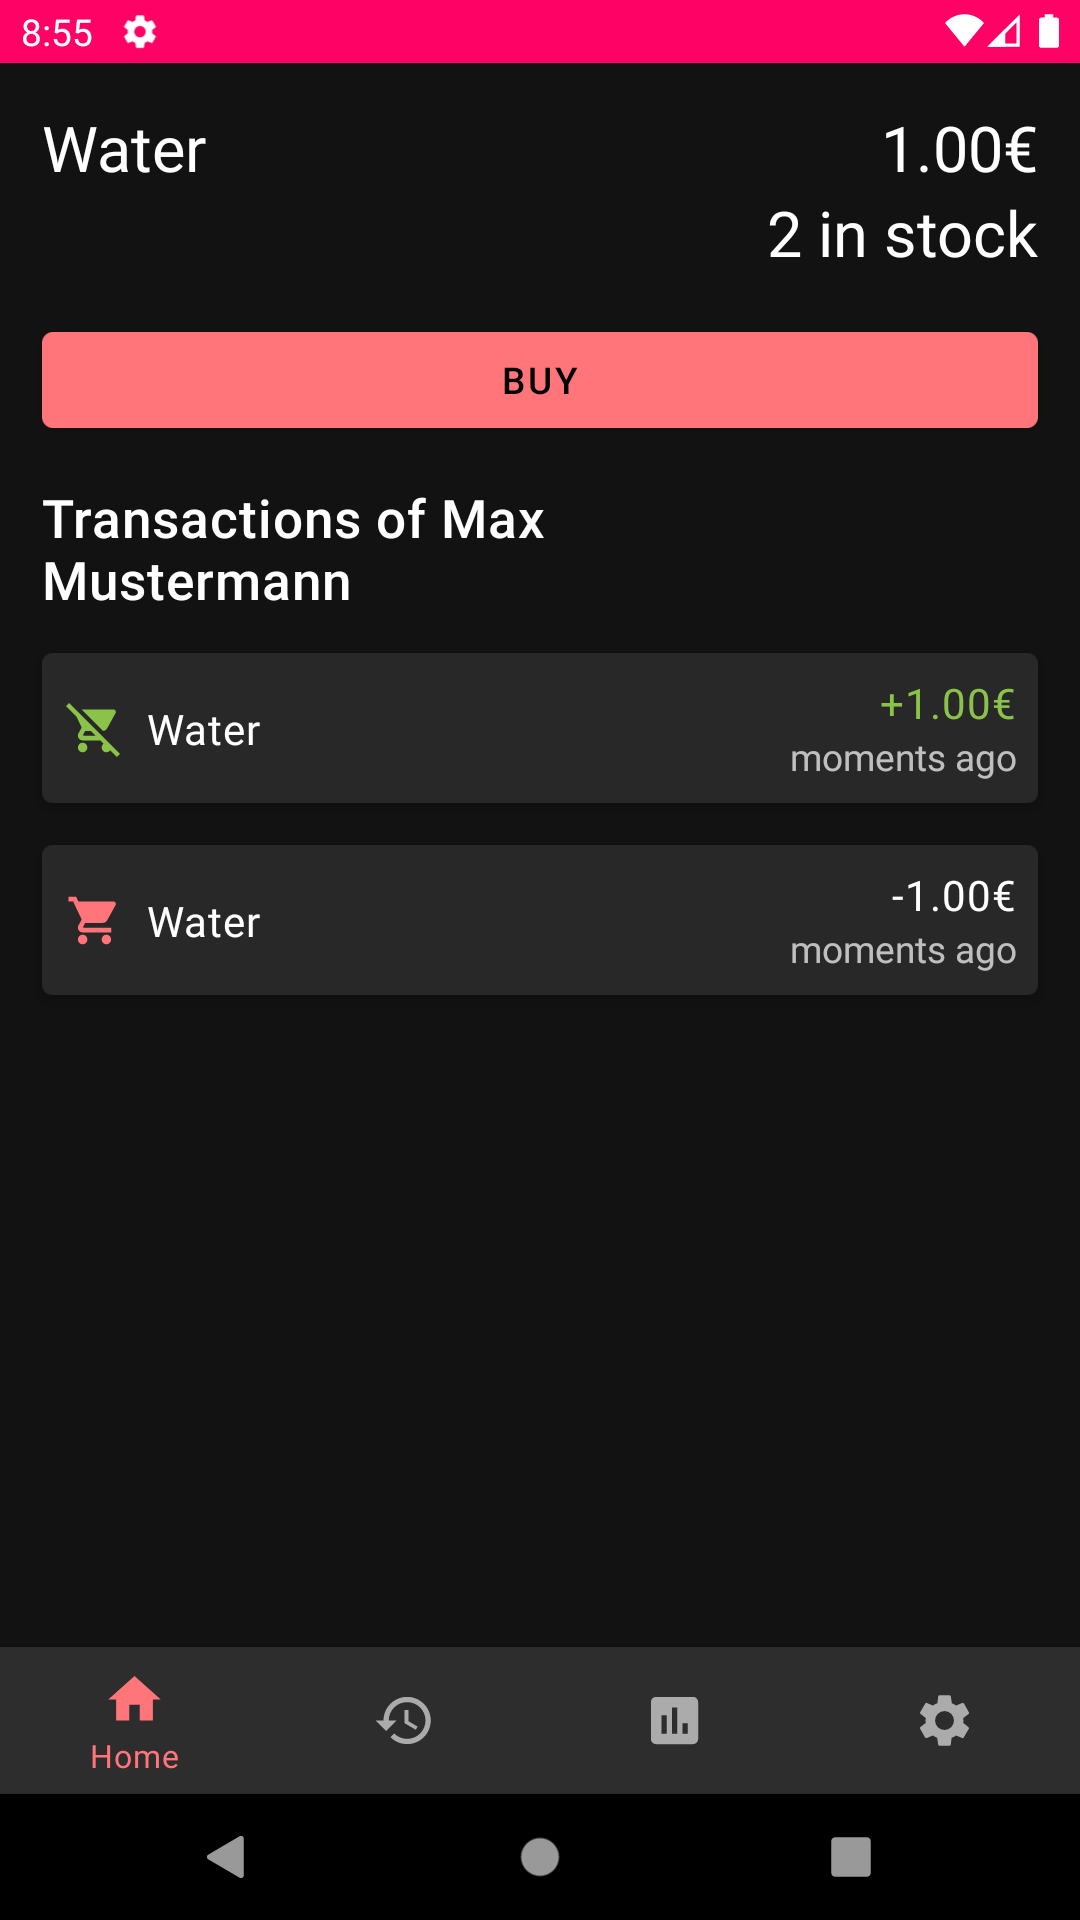
\includegraphics[height=8cm,keepaspectratio]{./img/screenshots/item-refunded.png}\label{fig:app:functionality:item:refund}}}%
	\caption{Artikelseite}%
	\label{fig:app:functionality:item}%
\end{figure}

Eine Übersicht über alle Transaktionen können sich Nutzer mit der Historie verschaffen.
Diese ist, wie auch Haupt-, Statistik- und Einstellungsseiten, über eine Navigationsleiste am unteren Bildschirmrand erreichbar.
Die Historie zeigt eine vollständige Liste aller Transaktionen, die der ausgewählte Nutzer getätigt hat.
Sie sind nach Transaktionszeitpunkten sortiert und geben Art, Wert und weitere Details der Transaktion an, wie in \autoref{fig:app:functionality:history:history} abgebildet ist.
Durch Klicken auf Käufe oder Stornierungen wird zur Seite des zugehörigen Artikels navigiert.
Wie bei allen Bildschirmen dieser App ist es zudem möglich die Seite durch eine \textit{Swipe-to-Refresh}-Geste zu aktualisieren.
Auf der Statistikseite finden sich Angaben zu Anzahl und letzten Kaufzeitpunkten pro Artikel vom aktiven Nutzer (siehe \autoref{fig:app:functionality:history:statistics}).
Auch hier ist es möglich, durch Klicken auf einen Eintrag zur Seite des zugehörigen Artikels zu navigieren.
\begin{figure}%
	\centering
	\subfloat{{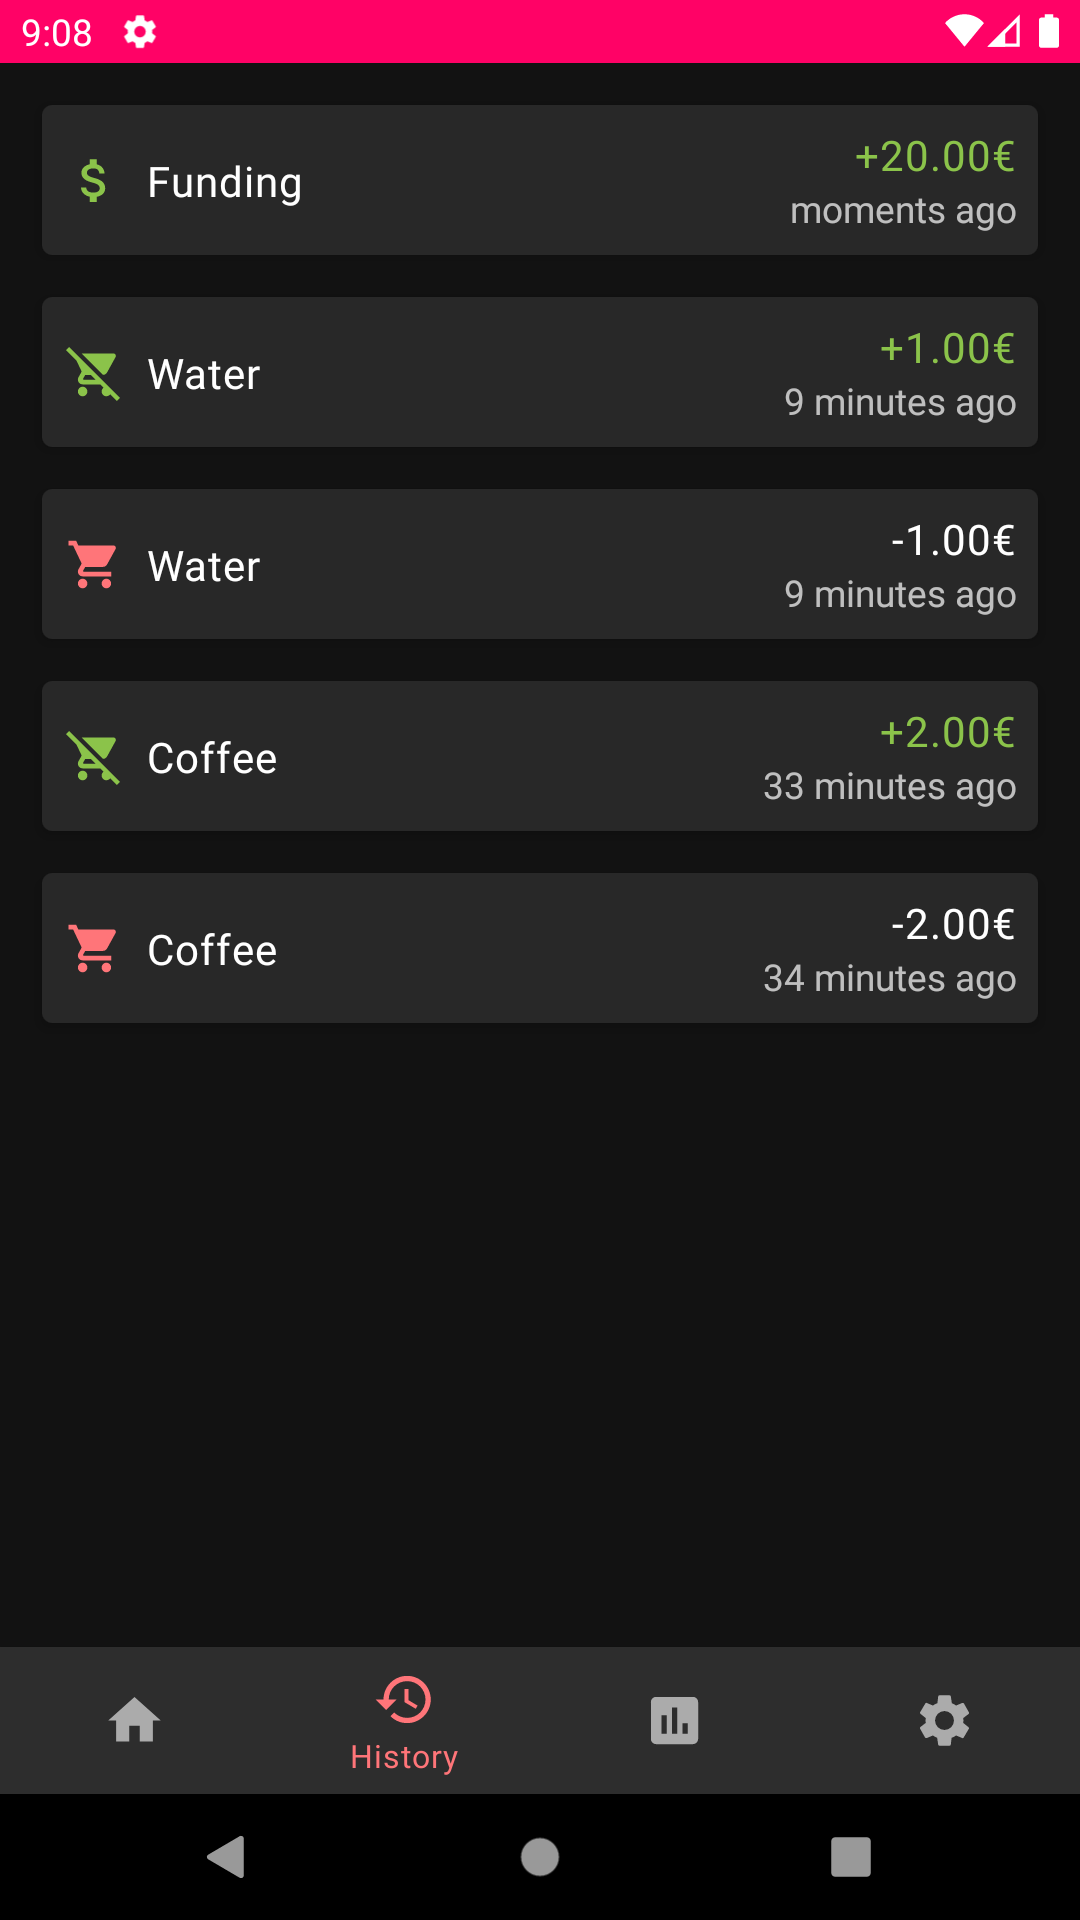
\includegraphics[height=8cm,keepaspectratio]{./img/screenshots/history.png}\label{fig:app:functionality:history:history}}}%
	\qquad
	\subfloat{{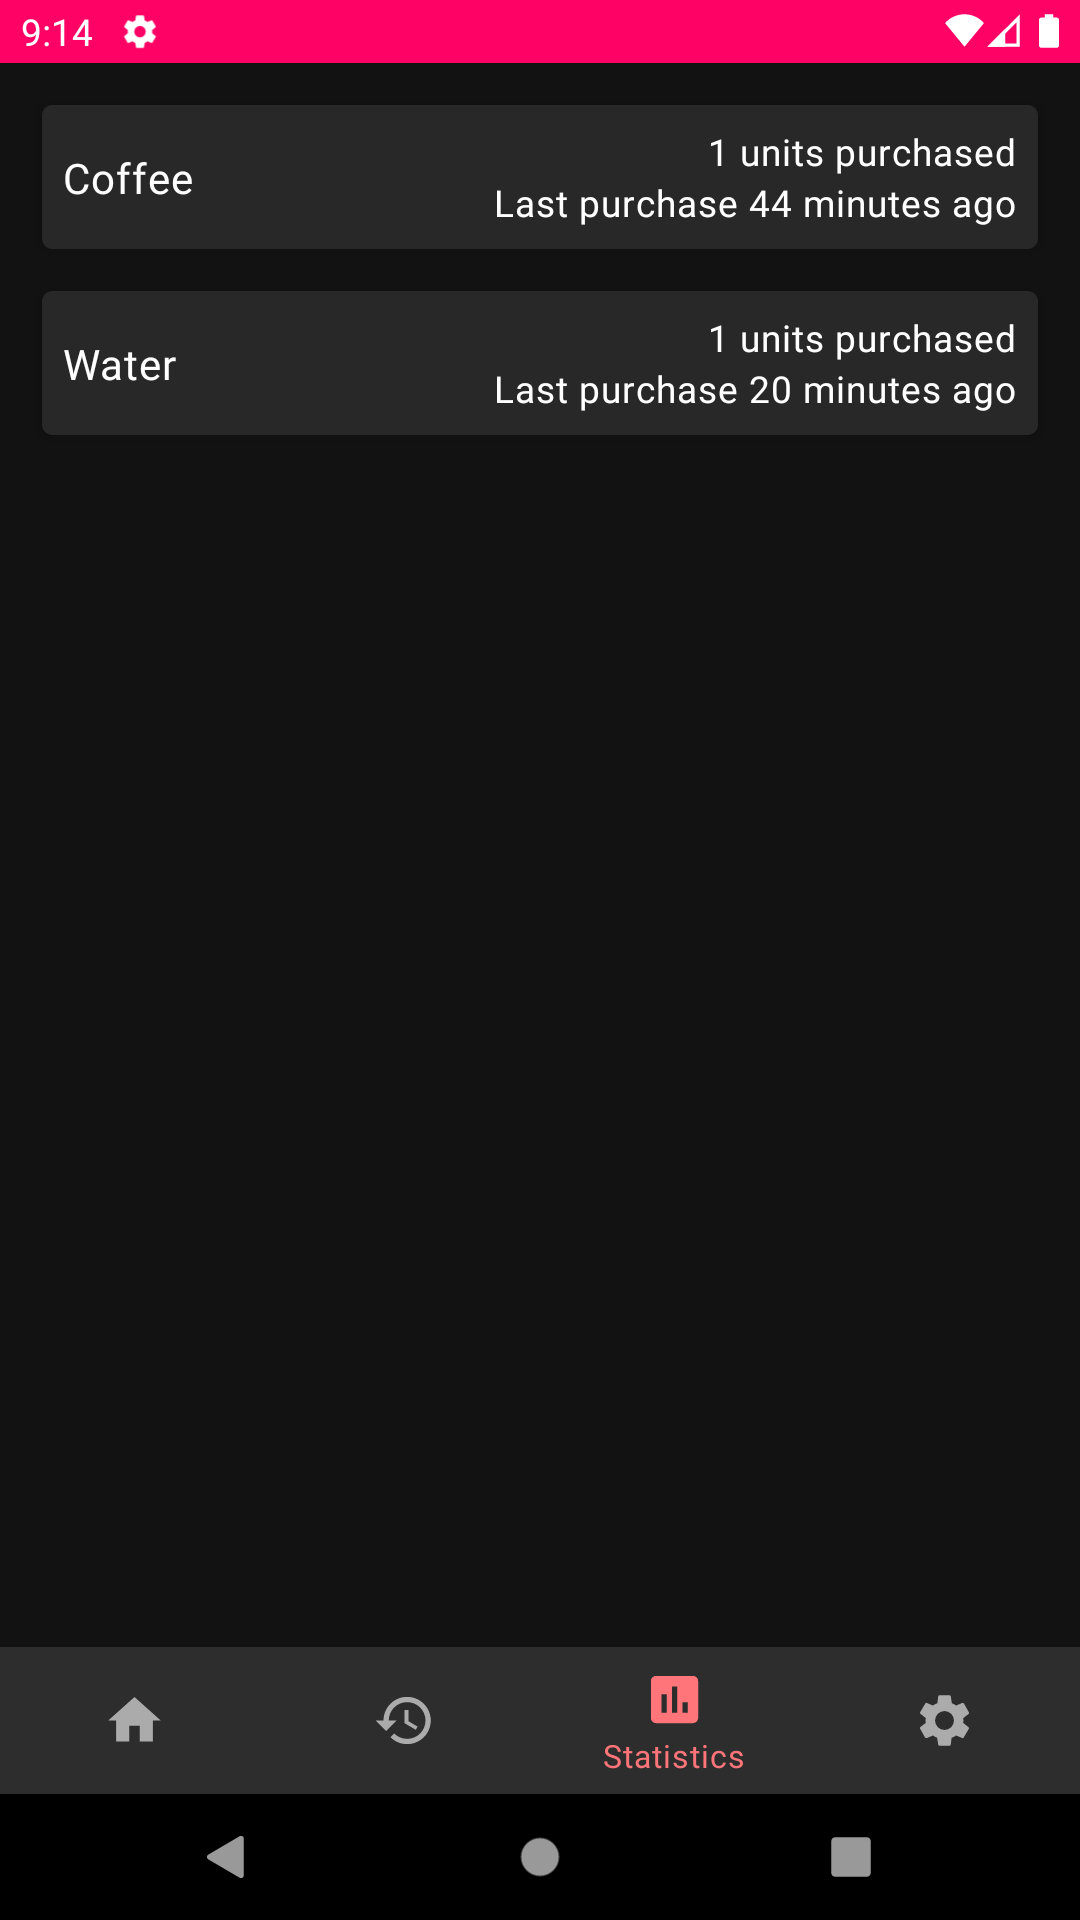
\includegraphics[height=8cm,keepaspectratio]{./img/screenshots/statistics.png}\label{fig:app:functionality:history:statistics}}}%
	\caption{Historie und Statistiken}%
	\label{fig:app:functionality:history}%
\end{figure}

Die Einstellungen umfassen neben Optionen zur erneuten Nutzerauswahl und Starten des geteilten Modus auch die Administrator-Funktionen (siehe \autoref{fig:app:functionality:settings:settings}).
Diese sind jedoch erst nach einem Login zugänglich, welcher über die in \autoref{fig:app:functionality:settings:login} gezeigte Seite stattfindet.
\begin{figure}%
	\centering
	\subfloat{{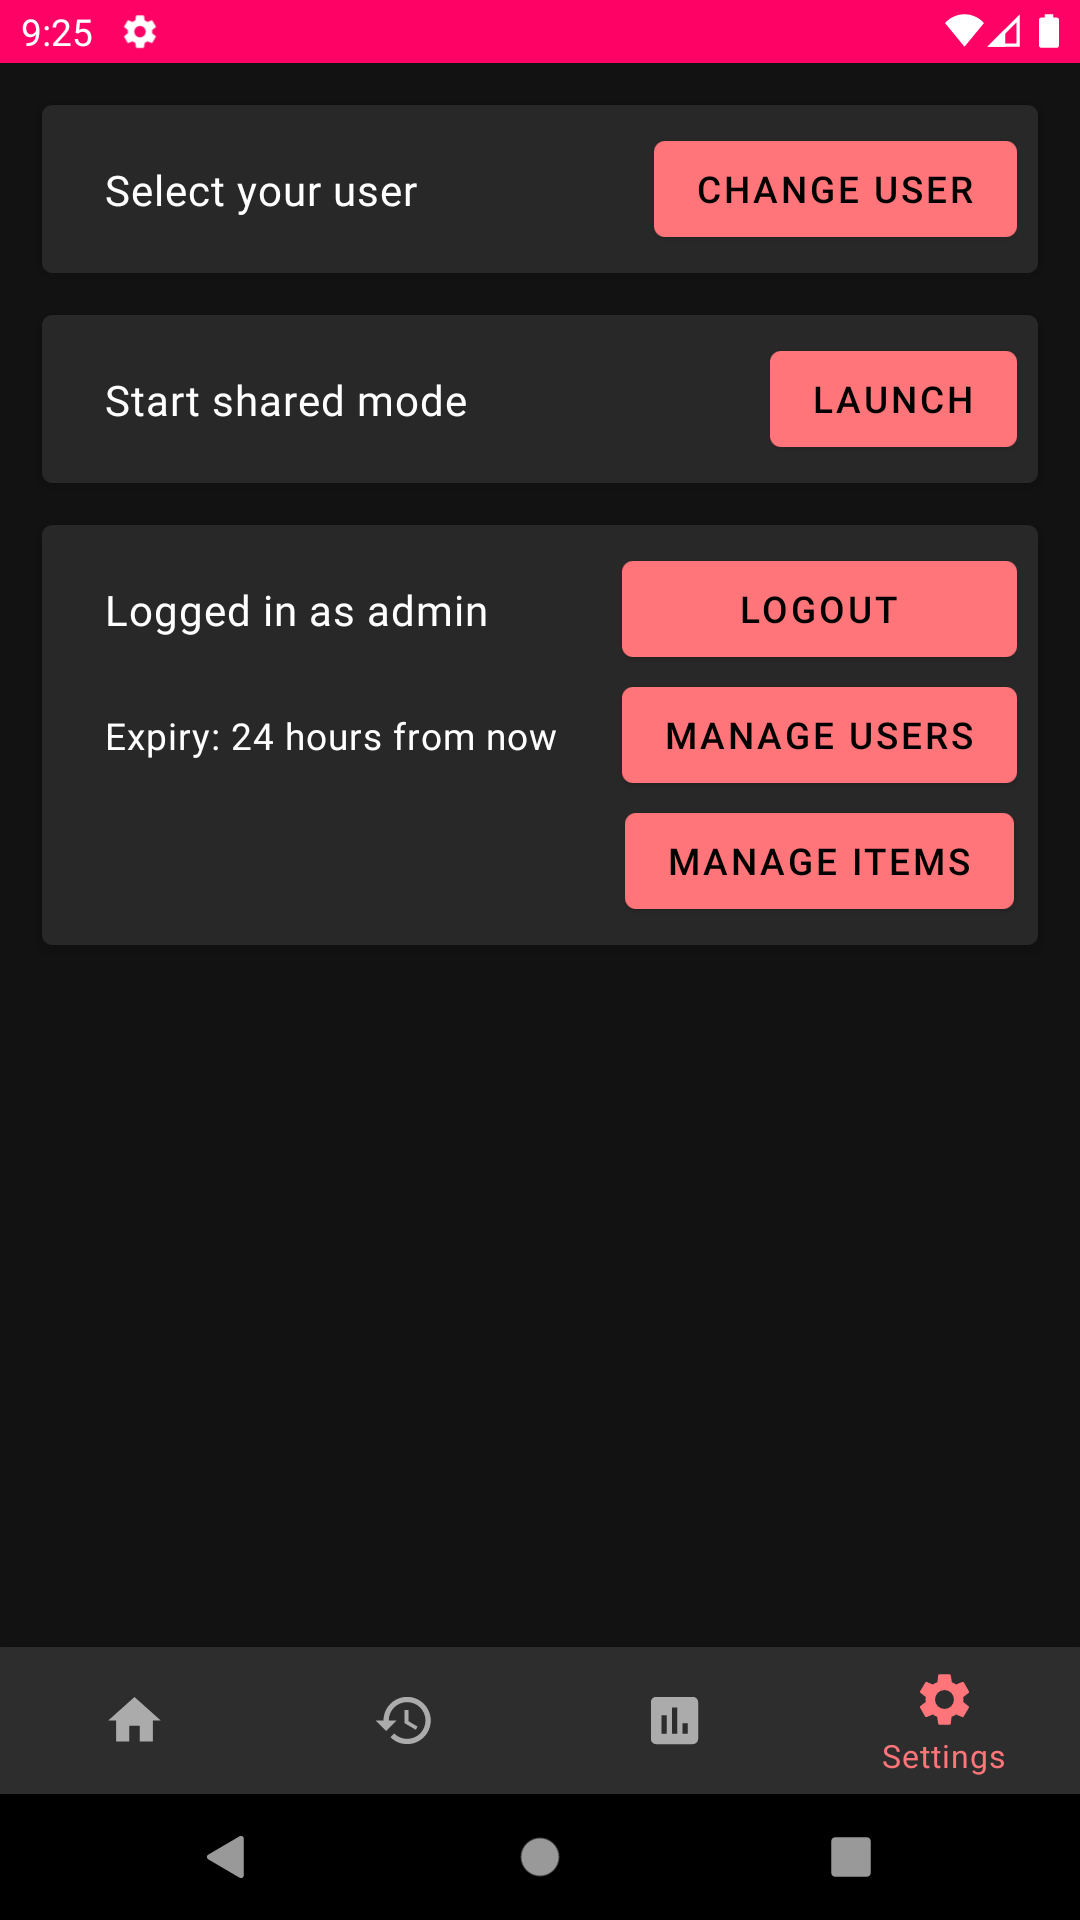
\includegraphics[height=8cm,keepaspectratio]{./img/screenshots/settings-admin.png}\label{fig:app:functionality:settings:settings}}}%
	\qquad
	\subfloat{{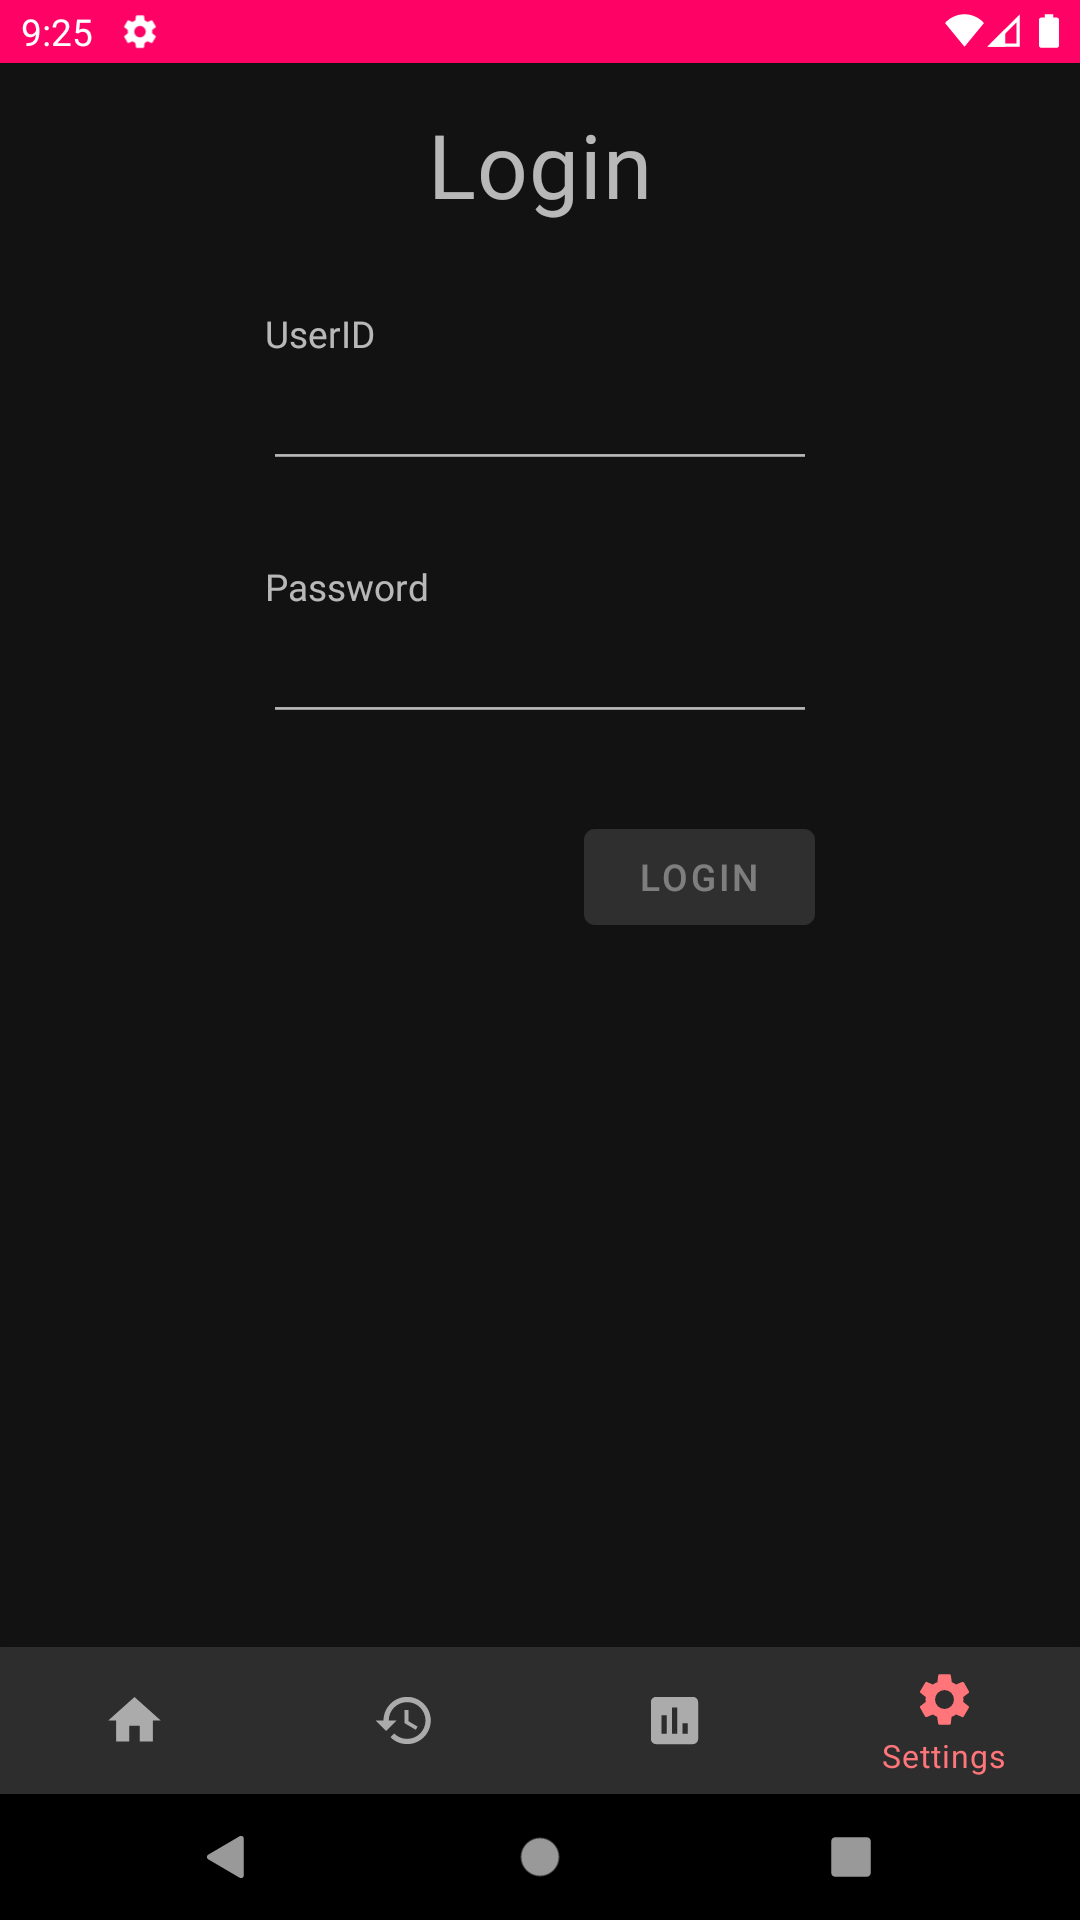
\includegraphics[height=8cm,keepaspectratio]{./img/screenshots/login.png}\label{fig:app:functionality:settings:login}}}%
	\caption{Einstellungen und Login}%
	\label{fig:app:functionality:settings}%
\end{figure}
Die Buttons \textit{MANAGE USERS} und \textit{MANAGE ITEMS} öffnen Seiten, welche jeweils denen der Nutzer- und Artikelauswahl entsprechen.
Sie verfügen jedoch über zusätzliche Buttons, die Seiten zum Erstellen neuer Nutzer beziehungsweise Artikel öffnen.
\autoref{fig:app:functionality:admin:create} zeigt die Nutzervariante dieser Seite.
Felder, welche als optional markiert sind, müssen nicht ausgefüllt werden.
IDs können beispielsweise von der Serveranwendung vergeben werden.
Um einen Nutzer oder Artikel zu bearbeiten muss auf diesen geklickt werden.
Während sich bei Artikeln eine erweiterte Ansicht der Artikelseite öffnet, haben Administratoren eine besondere Ansicht für Nutzer (siehe \autoref{fig:app:functionality:admin:user}).
Dort sehen sie alle Transaktionen, können Profilbildern bearbeiten sowie löschen und haben die Möglichkeit Guthaben aufzuladen.
Letzteres wird dann über eine eigene Seite, welche in \autoref{fig:app:functionality:admin:crediting} zu sehen ist, durchgeführt.
Sowohl bei Nutzern als auch bei Artikeln gibt es Optionen zum Löschen und Bearbeiten der gesamten Entität.
Aufbau der Bearbeitungsseiten entspricht denen der Seiten zum Erstellen, wie in \autoref{fig:app:functionality:admin:edit} zu sehen ist.
Beim Löschen müssen zwei Dialoge bestätigt werden um sicherzustellen, dass die Aktion bewusst stattfindet.
\begin{figure}%
	\centering
	\subfloat{{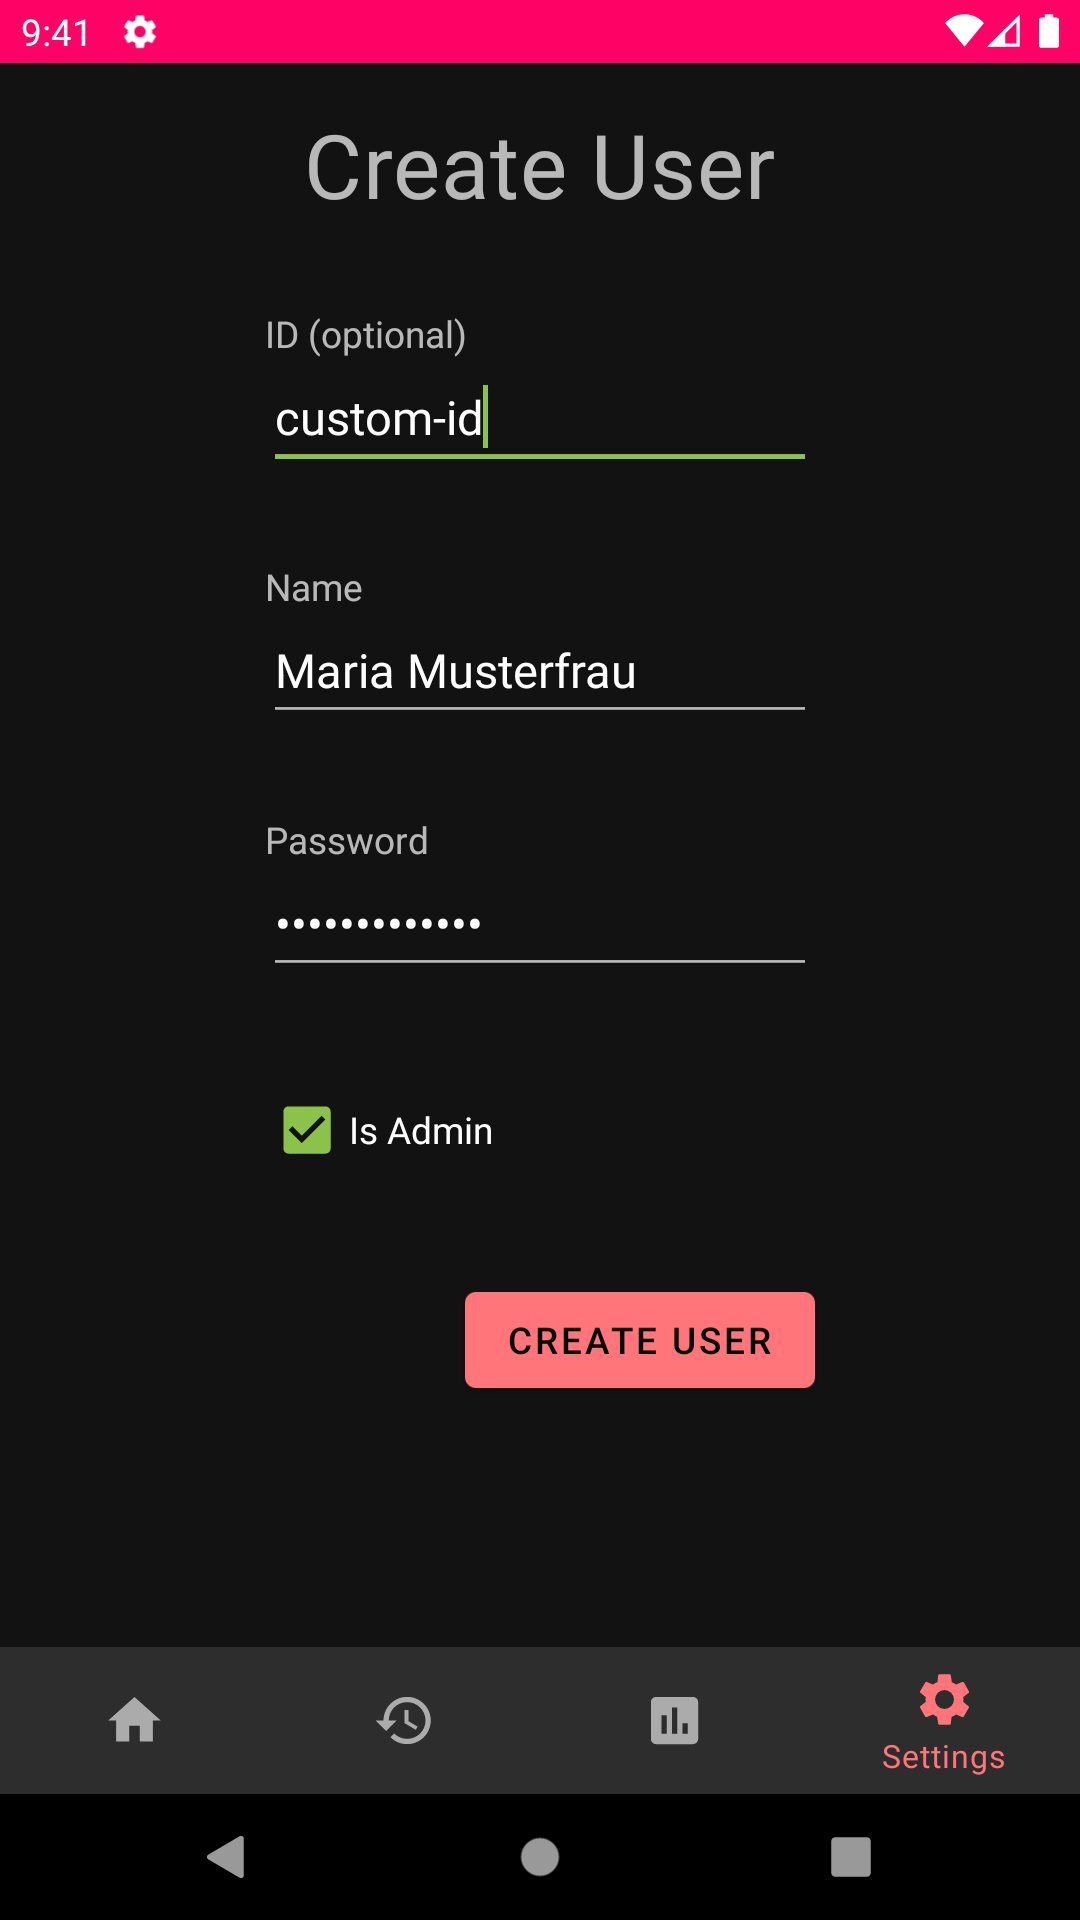
\includegraphics[height=8cm,keepaspectratio]{./img/screenshots/create-user.png}\label{fig:app:functionality:admin:create}}}%
	\qquad
	\subfloat{{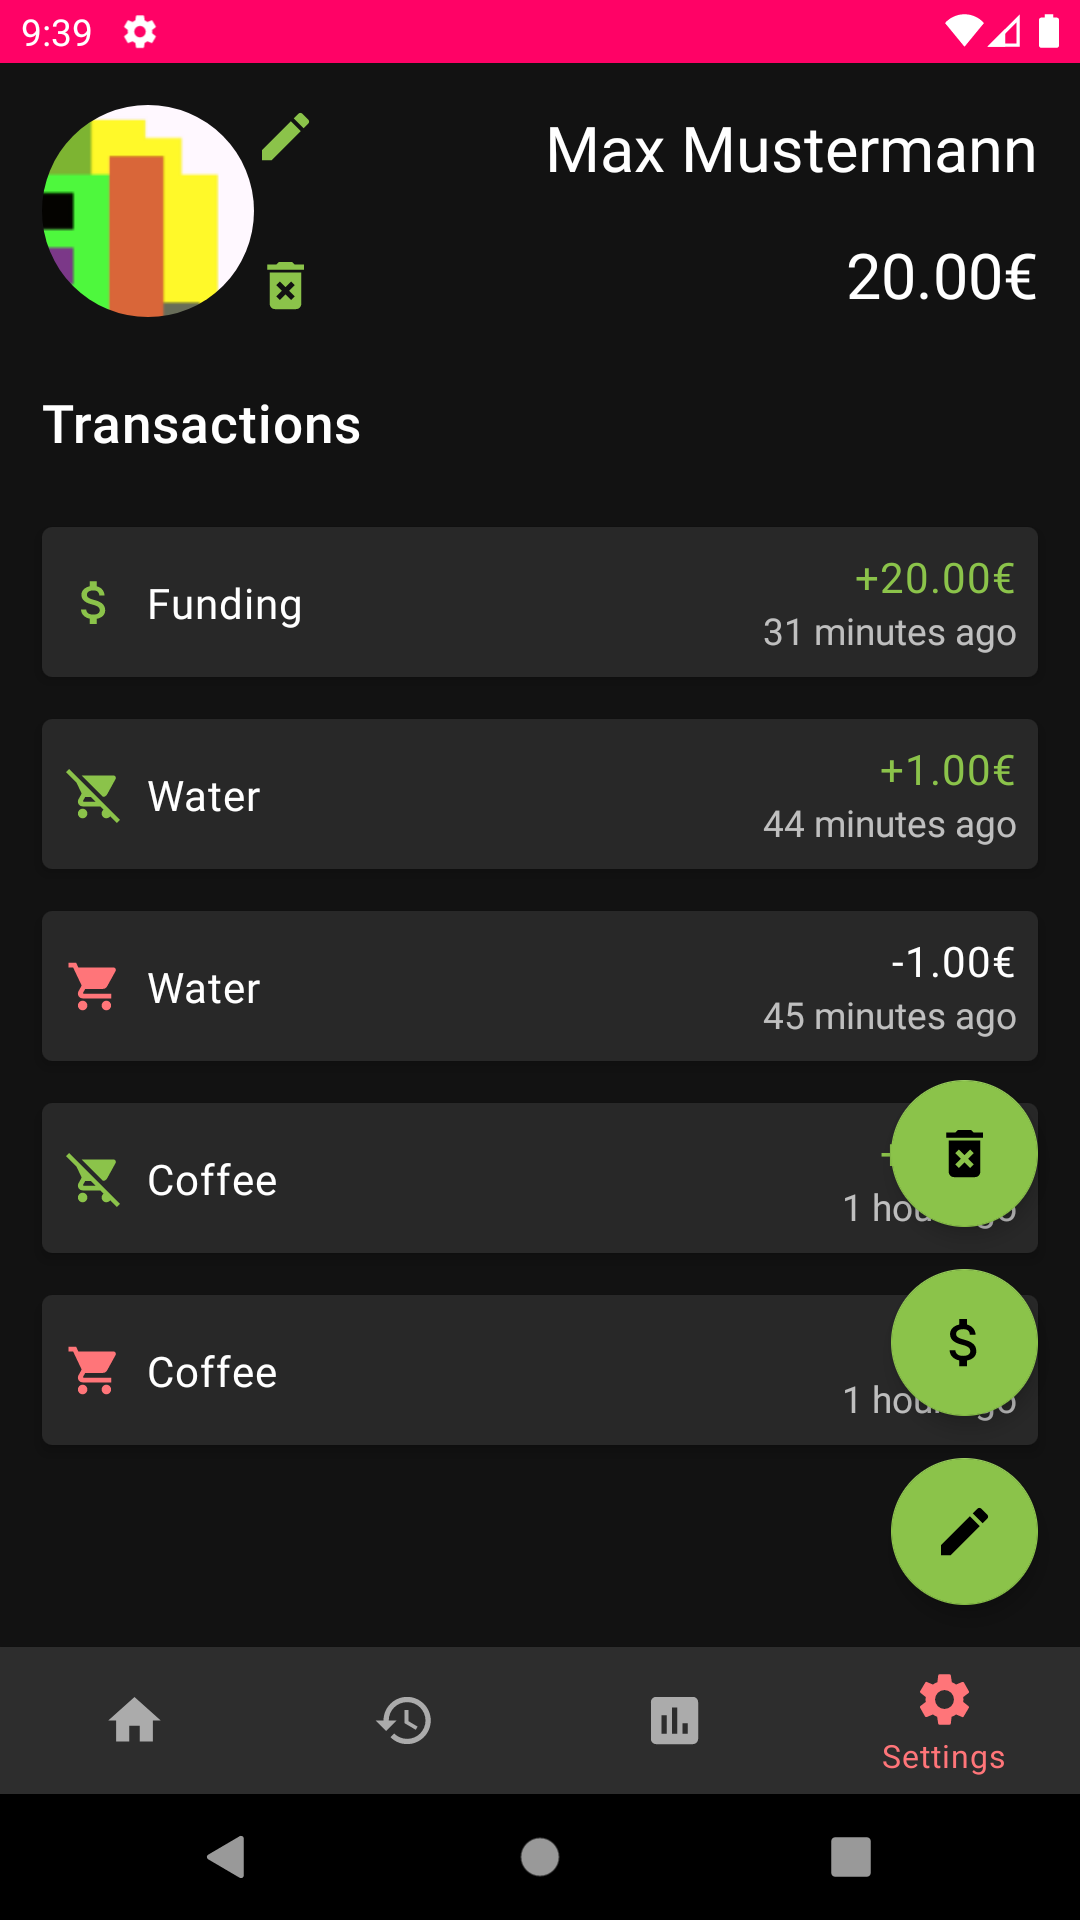
\includegraphics[height=8cm,keepaspectratio]{./img/screenshots/user-admin-view.png}\label{fig:app:functionality:admin:user}}}%
	\qquad
	\subfloat{{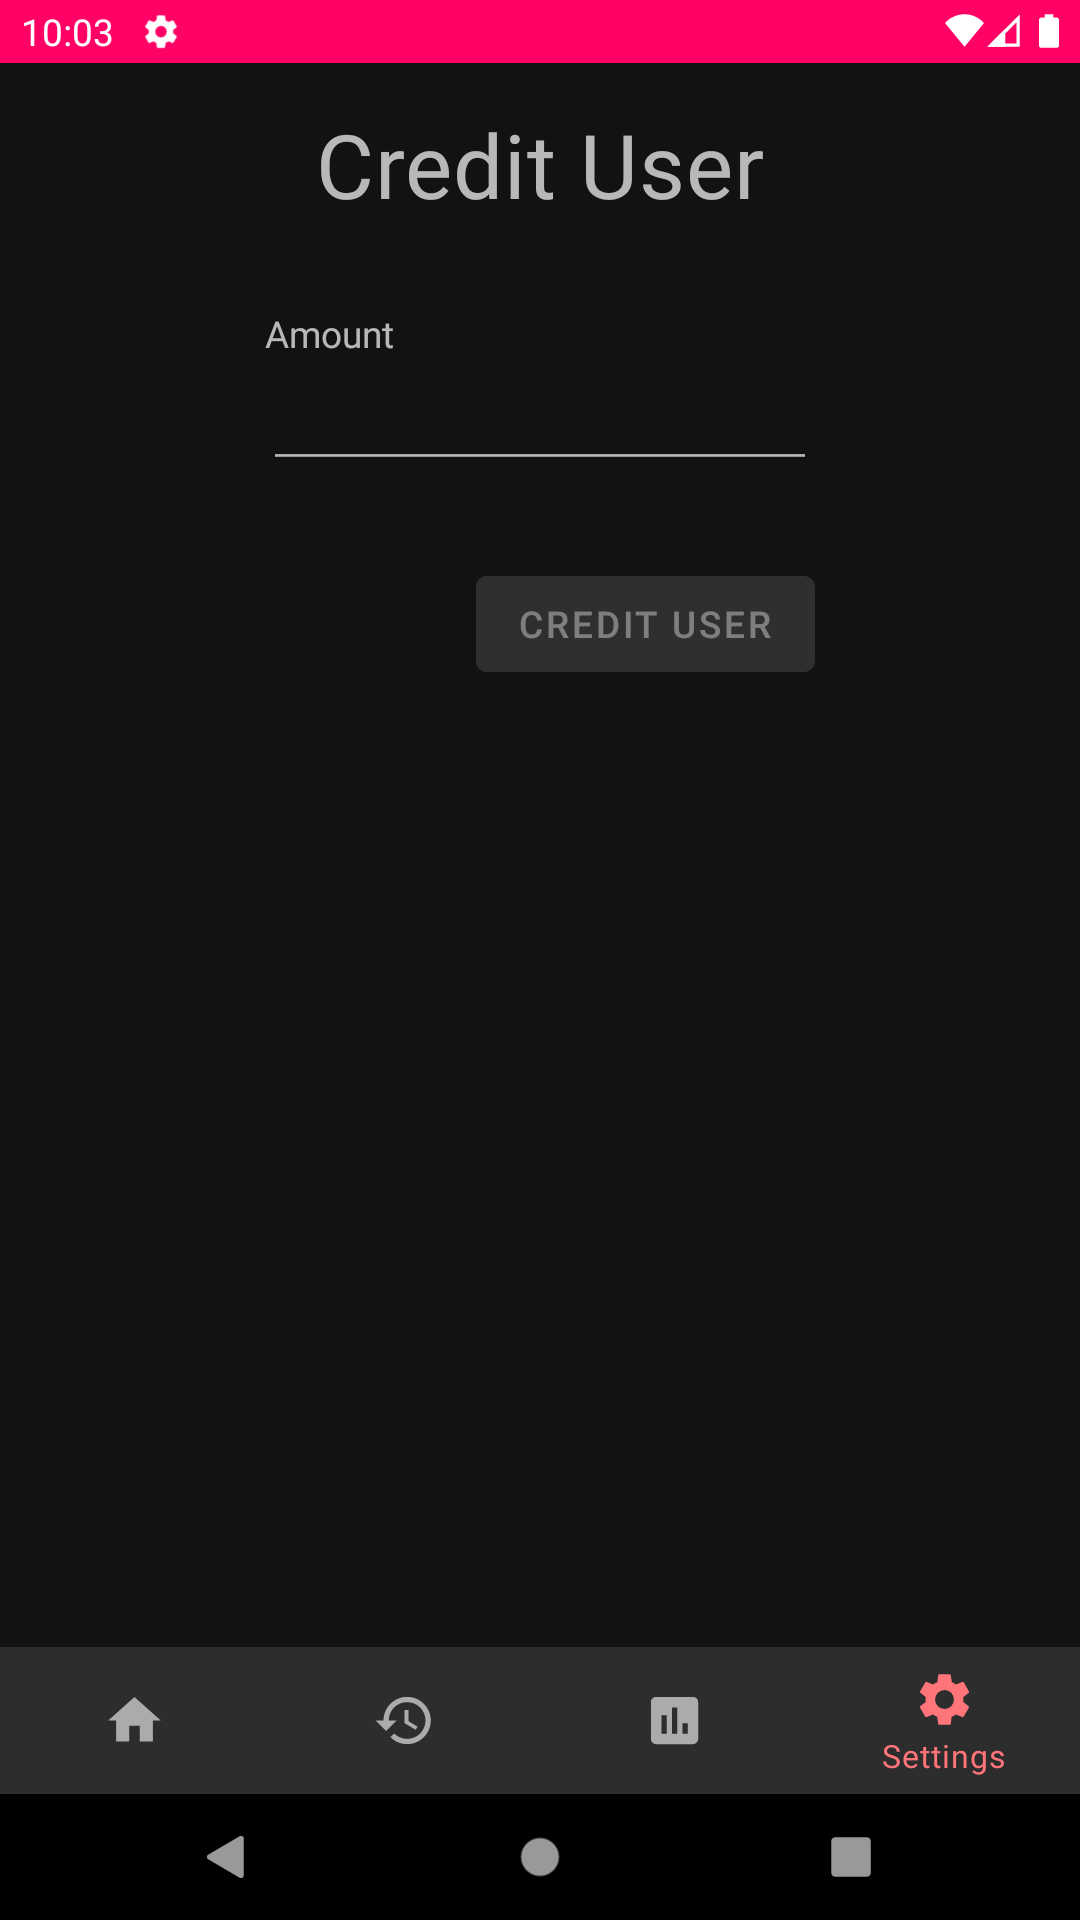
\includegraphics[height=8cm,keepaspectratio]{./img/screenshots/crediting.png}\label{fig:app:functionality:admin:crediting}}}%
	\qquad
	\subfloat{{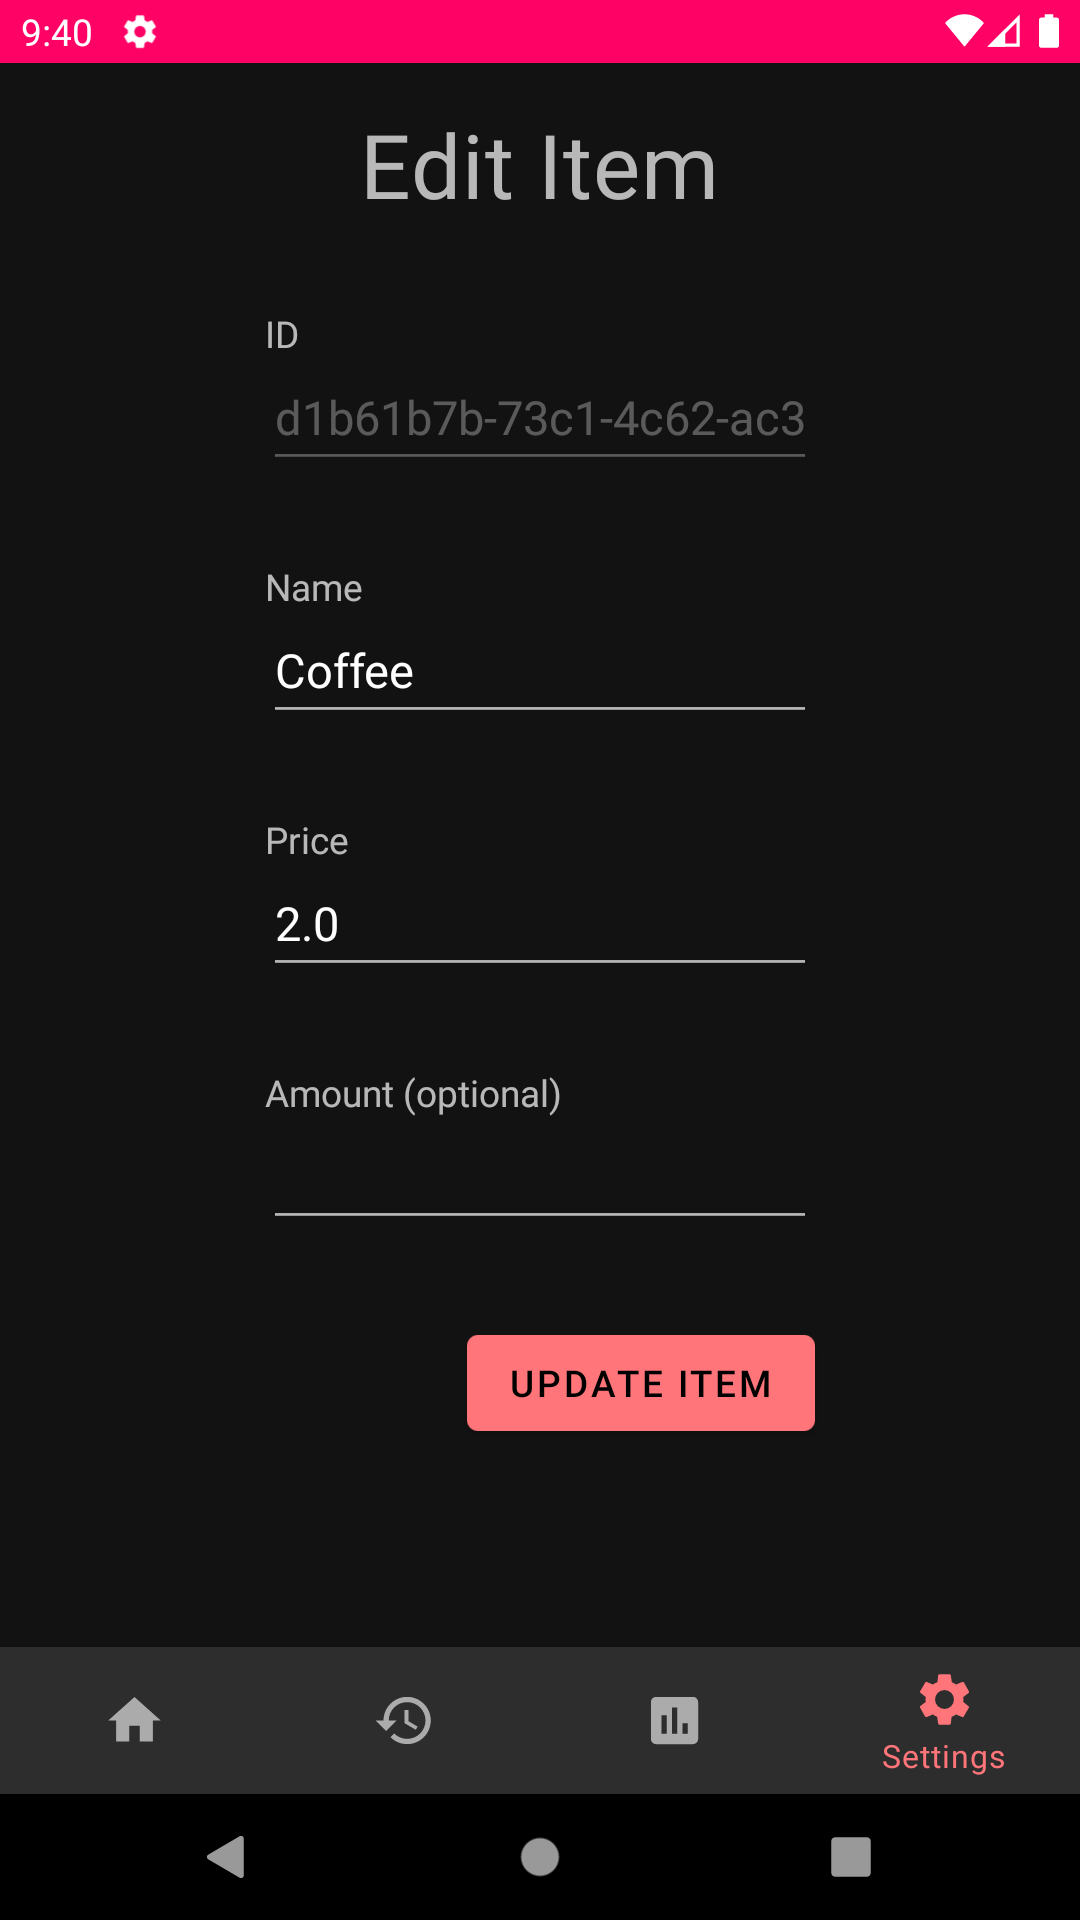
\includegraphics[height=8cm,keepaspectratio]{./img/screenshots/edit-item.png}\label{fig:app:functionality:admin:edit}}}%
	\caption{Administrator-Funktionen}%
	\label{fig:app:functionality:admin}%
\end{figure}

Der geteilte Modus dient dazu einen schnellen Nutzerwechsel zu ermöglichen.
Er umfasst ebenfalls Nutzerauswahl, Haupt- und Artikelseiten.
Es ist jedoch nur möglich in dieser Reihenfolge zwischen ihnen zu navigieren, da ausgewählte Nutzer nicht gespeichert werden.
Nachdem dieser Modus gestartet wurde, kann er nur durch einen Neustart der App wieder verlassen werden.

Sollten während einer Verwendung der App Fehler auftreten, werden Nutzer über einen Text am unteren Bildschirmrand darüber informiert.
Parallel werden Fehlerbehebungen, wie das Entfernen veralteter Daten, automatisch durchgeführt.
%------------------------------------------------------------------------------------------------------------------------------------------------------

\section{Architektur}
\label{sec:app:architecture}
Die App verwendet die von Google empfohlene \textit{Model-View-ViewModel} Architektur (\textit{MVVM}) \autocite{androidarchitecture}.
Bei dieser wird die Anwendung in Datenmodell, Benutzeroberfläche und die sogenannten \textit{ViewModels} aufgeteilt (siehe \autoref{fig:app:architecture:mvvm}).
MVVM wurde 2005 von Microsoft vorgestellt.
Ziel war es, Quelltext zum Verwalten von Benutzeroberflächen zu reduzieren und falls möglich gänzlich zu eliminieren.
Essentiell dafür ist das \textit{Binding}-Konzept (siehe \autoref{subsec:app:jetpack:databinding}).

Die Ebene des Datenmodells liegt in Form von \textit{Repositories} vor.
Diese kommunizieren über eine Netzwerkschnittstelle mit der Serveranwendung um Daten zu laden oder Aktionen wie Käufe und Logins durchzuführen.
So erhaltene Daten werden unmittelbar in die lokale Datenbank geschrieben und auch nur von dort aus geladen.
Über diesen Mechanismus wird eine lokale Persistenz ermöglicht, wodurch Daten auch ohne Verbindung zum Server angezeigt werden können.
Weil der Zustand eines Datenmodells ausschließlich vom zugehörigen Repository bestimmt wird, werden sie auch als \textit{Single source of truth} bezeichnet.
Durch diese Eigenschaft ist es möglich, inkonsistente Datenbestände zu verhindern.

ViewModels passen von Repositories bereitgestellte Daten für Benutzeroberflächen an und stellen sie in Datencontainern bereit.
Sie selbst haben keine Informationen über Benutzeroberflächen.
Stattdessen reagieren diese auf Änderungen an ViewModels und entscheiden selbst über die Datenanzeige.
Bei Android liegen Benutzeroberflächen in Form von Fragmenten und Activities vor.

Die strikte Trennung der Schichten ermöglicht ein Testen der Geschäftslogik, ohne Benutzeroberflächen zu verwenden.
Gleichzeitig ist es so möglich Logik unabhängig von der konkreten Benutzeroberfläche wiederzuverwenden.

\begin{figure}
	\centering
	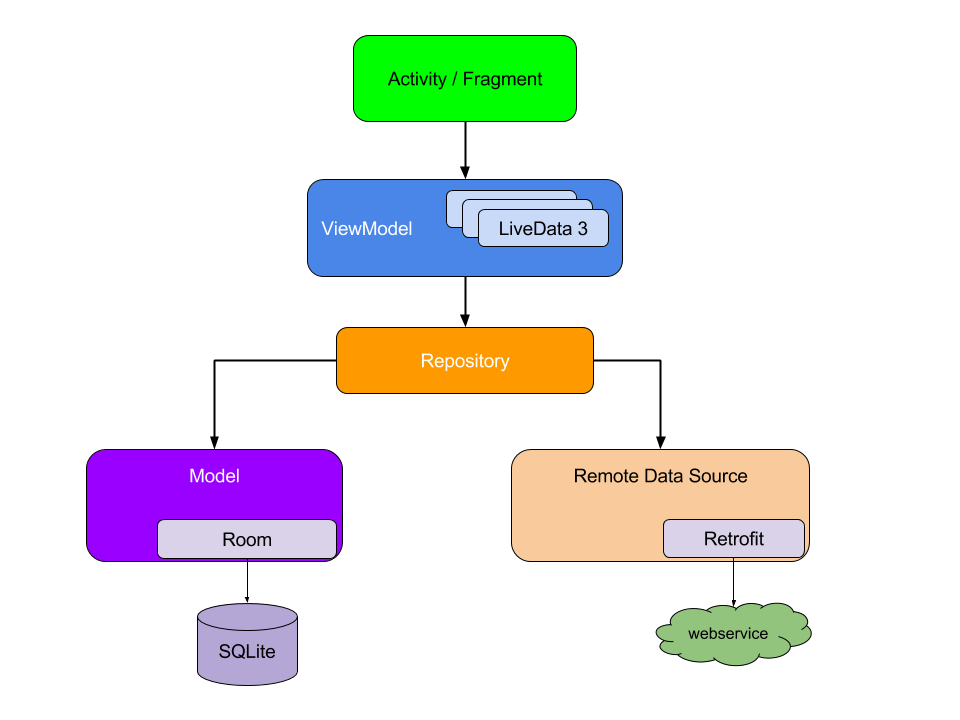
\includegraphics[height=8cm,keepaspectratio]{./img/android-architecture.png}
	\caption{MVVM-Entwurfsmuster in Android \autocite{androidarchitecture}}
	\label{fig:app:architecture:mvvm}
\end{figure}
%------------------------------------------------------------------------------------------------------------------------------------------------------

\section{Android Jetpack}
\label{sec:app:jetpack}
Android Jetpack umfasst eine Reihe von Bibliotheken, welche dazu dienen, die Entwicklung moderner Android Apps zu vereinfachen.
Dazu reduzieren sie beispielsweise den notwendigen \textit{Boilerplate Code} und vereinheitlichen Interaktionen mit dem Android Framework über verschiedene API Level hinweg.
Des Weiteren existieren Komponenten, welche bereits umfassende Grundlagen der MVVM-Architektur implementieren oder komplexe Elemente für Benutzeroberflächen bereitstellen.

Vor der Einführung von Jetpack mit Android 9.0 konnten Entwickler auf Support Libraries zurückgreifen.
Diese stellten bereits einen kleinen Teil der Jetpack Funktionalität zur Verfügung.
Sie unterscheiden sich jedoch dadurch, dass ihre Veröffentlichungen unterschiedliche API Level unterstützten \autocite{supportlibrariesversions}.
Dementsprechend konnten keine einheitliche Entwicklung über API Level hinweg ermöglichen.
Jetpack behebt dieses Problem, indem auf unterschiedliche Versionen für verschiedene API Level verzichtet wird.
Stattdessen wird Kompatibilität von Jetpack selbst sichergestellt, indem Interaktionen mit dem Android Framework verkapselt werden.
Die Entwicklungsumgebung Android Studio erstellt neue Projekte standardmäßig mit Jetpack.
Projekte, welche Support Libraries verwenden, können automatisch migriert werden, so dass Entwickler schnell und einfach umsteigen können \autocite{androidxmigration}.

Zum Zeitpunkt dieser Ausarbeitung existieren 82 Jetpack Bibliotheken, von denen ein Großteil produktionsbereite Veröffentlichungen besitzt \autocite{jetpackcount}.
Diese werden kontinuierlich aktualisiert, erweitert und durch neue Bibliotheken ergänzt.
Im Folgenden werden die in dieser App verwendeten Android Jetpack Bibliotheken kurz vorgestellt. Detaillierte Informationen können der offiziellen Dokumentation entnommen werden.
%------------------------------------------------------------------------------------------------------------------------------------------------------

\subsection{Core und AppCompat}
\label{subsec:app:jetpack:base}
Die \textit{Core} und \textit{AppCompat} Bibliotheken ermöglichen eine Verwendung von Funktionen neuer Android API Level auf älteren Android Versionen.
Dazu stellen sie eine Vielzahl an Hilfsklassen zur Verfügung, welche die unterschiedliche Behandlung der API Level verkapseln und die Entwicklung so vereinheitlichen und vereinfachen.
Die Klasse \textit{AppCompatActivity} erlaubt beispielsweise eine Verwendung von \textit{ActionBars}, welche ohne sie auf älteren Android Versionen nicht möglich wäre.
Core enthält hingegen Kompatibilitätskomponenten, welche Benachrichtigungen, Berechtigungen und weitere Interaktionen mit dem Android Framework über API Level hinweg vereinheitlichen.
%------------------------------------------------------------------------------------------------------------------------------------------------------

\subsection{Fragment}
\label{subsec:app:jetpack:fragment}
Fragmente sind modulare Teile von Benutzeroberflächen.
Sie sind wiederverwendbar, leichtgewichtig und lassen sich in \textit{Activities} sowie anderen Fragmenten kombinieren um komplexe Benutzeroberflächen zu erstellen.
Ihr Lebenszyklus wird vom Android Framework verwaltet, weshalb Entwickler für diesen keinen Mehraufwand betreiben müssen.
Darüber hinaus ist es möglich, Fragmente dynamisch hinzuzufügen und zu entfernen.
Komplexe \textit{Layouts} lassen sich so in mehrere Fragmente unterteilen, welche unabhängig voneinander wiederverwendbar sind.
%------------------------------------------------------------------------------------------------------------------------------------------------------

\subsection{Databinding}
\label{subsec:app:jetpack:databinding}
Mithilfe der \textit{Databinding} Bibliothek ist es möglich, Datenquellen für Eigenschaften von Benutzeroberflächen und deren Elemente, welche auch \textit{Views} genannt werden, in Layout-Dateien festzulegen.
Dafür werden sogenannte \textit{BindingImplementations} generiert, welche die dafür benötigte Logik bereitstellen und zudem direkte Zugriffe auf Views ermöglichen.
In Kombination mit \textit{LiveData} passen sich Benutzeroberflächen bei Änderungen automatisch an, wodurch der Anteil an Quelltext für Benutzeroberflächen reduziert wird.
Zusätzlich lassen sich \textit{BindingAdapters} definieren.
Dabei handelt es sich um Funktionen, welche eine View sowie weitere beliebige Parameter erhalten.
Sie können in Layout-Dateien verwendet werden um benutzerdefiniertes Verhalten sowie Eigenschaften zu definieren.
Zum Beispiel kann ein BindingAdapter definiert werden, welcher in Abhängigkeit eines Parameters Views aus- und einblendet.
%------------------------------------------------------------------------------------------------------------------------------------------------------

\subsection{Lifecycle}
\label{subsec:app:jetpack:lifecycle}
Die \textit{Lifecycle} Bibliothek umfasst primär ViewModels und LiveData, aber auch allgemeine Komponenten zum Verwalten und Implementieren von Lebenszyklen.

Jetpack ViewModels werden vom Android Framework verwaltet.
Sie besitzen einen Lebenszyklus, welcher sich Fragmenten anpasst, die ihre Instanzen verwenden.
So kann sichergestellt werden, dass sie nach einer Zerstörung zugehöriger Fragmente korrekt beendet werden.

LiveData baut auf diesem Konzept auf.
Dabei handelt es sich um \textit{Wrapper} für beliebige Daten, deren Werte beobachtet werden können.
Anders als traditionelle \textit{Observables} besitzt LiveData jedoch einen Lebenszyklus.
Sobald keine \textit{Oberserver} mehr registriert sind, da deren Lebenszyklus beendet wurde, propagiert LiveData keine Änderungen mehr.
Entwickler müssen deshalb keine Referenzen entfernen oder auf andere Art und Weise sicherstellen, dass ihre Observables korrekt terminiert werden.
LiveData übernimmt diesen Aspekt, welcher bei inkorrekter Behandlung leicht zu \textit{Memory Leaks} führen kann.
%------------------------------------------------------------------------------------------------------------------------------------------------------

\subsection{Navigation}
\label{subsec:app:jetpack:navigation}
Fragmente können mit Argumenten erzeugt werden.
Dabei ist jedoch keine Typsicherheit garantiert und es gibt keinen Mechanismus, der die Vollständigkeit von Argumenten sicherstellt.
Die \textit{Navigation} Bibliothek löst beide Probleme durch Navigationsgraphen.
In diesen werden verfügbare Fragmente und ihre Argumente festgelegt.
Durch Verbindungen zwischen Fragmenten werden \textit{Directions} definiert, welche Navigationsrichtungen symbolisieren.
Deren Verwendung bei der Navigation stellt sicher, dass alle Argumente mit korrektem Typ vorhanden sind und zum korrekten Fragment navigiert wird.
Zudem kann über Directions das Verhalten einer Navigation festgelegt werden.
Darunter fallen beispielsweise Übergangsanimationen und ein Aufräumen des \textit{Android Backstacks}\footnote{Siehe \url{https://developer.android.com/guide/components/activities/tasks-and-back-stack}.}.
Darüber hinaus unterstützt die Bibliothek Navigationscontroller, die das Initialisieren von Benutzerelementen wie \textit{Bottom Navigations}, \textit{Hamburger Menus} und \textit{Toolbars} übernehmen.

%------------------------------------------------------------------------------------------------------------------------------------------------------

\subsection{ConstraintLayout und SwiperefreshLayout}
\label{subsec:app:jetpack:layouts}
Android Jetpack umfasst auch mehrere Layout-Bibliotheken.
Im Rahmen dieses Projektes wurden \textit{ConstraintLayout} und \textit{SwiperefreshLayout} verwendet.

Komplexe Hierarchien in Benutzeroberflächen verringern deren Performanz bei Layoutänderungen.
ConstraintLayout ermöglicht ein freies Platzieren von Views, durch relative Angaben zur Einschränkung ihrer Positionen.
Dies funktioniert, da Einschränkungen relativ zum Container als auch anderen Views angegeben werden können.
Auf Grund der flachen Hierarchie von ConstraintLayouts ist ihre Performanz deutlich besser als die alternativer Layouts \autocite{viewperformance}.
Gleichzeitig können sich so erstelle Layouts an unterschiedliche Bildschirmgrößen und -orientierungen anpassen, wodurch Benutzeroberflächen flexibler entwickelt werden können.

Bei mobilen Anwendungen gibt es die gängige \textit{Swipe-to-Refresh}-Geste zum Aktualisieren eines Bildschirms.
Mithilfe von SwiperefreshLayout ist es möglich, diese Funktionalität mit wenigen Zeilen Quelltext zu bestehenden Benutzeroberflächen hinzuzufügen.
SwiperefreshLayout verfügt über die von vielen Google Apps verwendete Spinner Animation und ist mit scrollbaren Views und Layouts kompatibel.
%------------------------------------------------------------------------------------------------------------------------------------------------------

\subsection{RecyclerView}
\label{subsec:app:jetpack:recyclerview}
\textit{RecyclerViews} ermöglichen ein Anzeigen von langen Listen, ohne dass Speicherverbrauch oder Performanz leiden.
Dies ist möglich, indem nicht mehr Container für Listenelemente erzeugt werden, als gleichzeitig darstellbar sind. 
Zudem werden sie für andere Listenelemente wiederverwendet, sobald sie nicht mehr sichtbar sind.
Durch dieses Konzept sind RecyclerViews performanter als beispielsweise \textit{ListViews} oder \textit{LinearLayouts}.
Zur Interaktion mit RecyclerViews werden Adapter verwendet, welche Erzeugen von Container und Zuweise von Elementen definieren.
Es stehen Hilfsklassen bereit, die bereits über einen Großteil der benötigten Logik verfügen.
\textit{ListAdapter} ermöglicht beispielsweise eine direkte Übergabe von Listen.
Um Änderungen an Listeneinträgen zu erkennen werden in der Regel \textit{DiffCallbacks} verwendet.
Diese sind in der Bibliothek enthalten und verwenden komplexe Algorithmen um Änderungen an Listen darzustellen, so dass nur betroffene Container aktualisiert werden müssen.
%------------------------------------------------------------------------------------------------------------------------------------------------------

\subsection{Room}
\label{subsec:app:jetpack:room}
Bei \textit{Room} handelt es sich um eine Abstraktionsebene für \textit{SQLite} Datenbanken.
Datenbankinteraktionen werden dabei in \textit{Data Access Objects}, auch \textit{DAOs} genannt, über Annotationen an Funktionen definiert.
Bei DAOs handelt es sich um \textit{Interfaces}, deren Implementierungen von Room generiert werden.
Komplexe SQL-Anfragen können ebenfalls in Textform angegeben werden.
Die Hauptfunktion von Room liegt jedoch in der Möglichkeit Rückgabewerte in reaktiven Wrapper-Klassen, wie beispielsweise LiveData, zu erhalten.
Room übernimmt in diesem Fall die Aktualisierung der Daten, wodurch es reicht Datenbankanfragen einmalig auszuführen.
Darüber hinaus können Datenbanktransaktionen programmatisch definiert und Konfliktstrategien an Voraussetzungen angepasst werden.
Room unterstützt zudem benutzerdefinierte Migrationsstrategien, wodurch Aktualisierungen von Datenbankschemas erleichtert werden.
%------------------------------------------------------------------------------------------------------------------------------------------------------

\subsection{Paging}
\label{subsec:app:jetpack:paging}
Das Laden großer Datenmengen aus Datenbanken oder Netzwerkquellen ist ein nicht zu unterschätzender Aufwand.
Die \textit{Paging} Bibliothek ermöglicht deshalb ein stückweises Laden von Datensätzen.
Dazu muss eine \textit{DataSource Factory} vorliegen, welche dieses Konzept unterstützt.
Unter anderem ermöglicht Room solche \textit{Factories} als Rückgabewerte zu definieren.
Sie lassen sich zu LiveData Objekten transformieren, welche \textit{PagedLists} enthalten.
Diese besonderen Listen lassen sich unter anderem mit RecyclerViews und \textit{PagedListAdaptern} verwenden.
Im Endeffekt können so Performanz und Speicherverbrauch verbessert werden.
%------------------------------------------------------------------------------------------------------------------------------------------------------

\subsection{Work}
\label{subsec:app:jetpack:work}
Hintergrundaufgaben, wie beispielsweise das Bereinigen von Datenbanken, können über die \textit{Work} Bibliothek verwaltet werden.
Die zu erledigende Arbeit wird in \textit{Worker}-Klassen definiert, welche optional Coroutines verwenden können um vollständig asynchron ausgeführt zu werden.
Beim Registrieren von Worker-Instanzen können Einschränkungen definiert werden, welche Zustände, Zeitpunkte und Intervalle von Ausführungen festlegen.
So kann sichergestellt werden, dass beispielsweise eine Internetverbindung besteht oder Akkus von Endgeräten nicht übermäßig stark belastet werden.
Im Endeffekt erlaubt die Bibliothek so eine benutzerfreundliche Ausführung von Aufgaben, welche im Hintergrund stattfinden sollen.
%------------------------------------------------------------------------------------------------------------------------------------------------------

\subsection{KTX}
\label{subsec:app:jetpack:extensions}
Kotlin ist die von Google empfohlene Sprache für Android-Entwicklung \autocite{androidkotlin}.
Sie zeichnet sich unter anderem dadurch aus, dass sie im Vergleich zu Java deutlich weniger verbos und in der Regel entsprechend kürzer ist.
Eine Vielzahl an Android Jetpack Bibliotheken liegen in \textit{KTX}-Varianten vor.
Diese enthalten zusätzliche Erweiterungsmethoden und Sprachfunktionen, welche die Programmierung von Android Apps mit Kotlin vereinfachen.
Dazu zählen beispielsweise Erweiterungsmethoden, welche den Lesefluss von Aufrufen verbessern oder mehrere Methodenaufrufe zusammenfassen.
Des Weiteren existieren zahlreiche Methoden zum Erzeugen von ViewModels und LiveData, welche einen Großteil der Konfiguration verkapseln.
Auch Kotlin-spezifische Sprachkonstrukte wie \textit{Delegated Properties} und \textit{Coroutines} werden von Jetpack unterstützt, um die Entwicklung mit Kotlin weiter zu verbessern.
%------------------------------------------------------------------------------------------------------------------------------------------------------

\section{Weitere Bibliotheken}
\label{sec:app:bibs}
Im Rahmen der App-Entwicklung wurden auch Bibliotheken verwendet, welche nicht Teil von Android Jetpack sind.
Im Folgenden werden ihre Funktionen und Verwendungsgründe vorgestellt.
%------------------------------------------------------------------------------------------------------------------------------------------------------

\subsection{Retrofit und Moshi}
\label{subsec:app:bibs:retrofitmoshi}
Über \textit{Retrofit} können abstrakte Methoden zum Anbinden von APIs definiert werden.
Entwickler müssen dazu Informationen über die Art von Anfragen angeben.
Implementierungen dieser Methoden werden von der Bibliothek generiert.
In Kombination mit der Serialisierungsbibliothek \textit{Moshi} können so Netzwerkschnittstellen mit geringem Quelltextaufwand angebunden werden.
%------------------------------------------------------------------------------------------------------------------------------------------------------

\subsection{Glide}
\label{subsec:app:bibs:glide}
\textit{Glide} übernimmt das asynchrone Laden und Darstellen von Bildern.
Dabei lassen sich Einstellungen für Verhalten und Darstellung anpassen.
Unter anderem kann Glide Bilder für schnelleres Laden zwischenspeichern, zuschneiden und während einem Ladevorgang durch Platzhalter ersetzen.
%------------------------------------------------------------------------------------------------------------------------------------------------------

\subsection{Image Picker}
\label{subsec:app:bibs:imagepicker}
Die Bibliothek \textit{Image Picker} ermöglicht die Auswahl von Bildern zur Laufzeit, die Nutzer entweder aus ihrer Galerie auswählen oder mit ihrer Kamera aufnehmen können.
Eine äquivalente Funktionalität zu implementieren ist mit nicht-trivialem Aufwand verbunden, weshalb eine Verwendung existierender Bibliotheken die Entwicklung verkürzte.
%------------------------------------------------------------------------------------------------------------------------------------------------------

\subsection{PrettyTime}
\label{subsec:app:bibs:prettytime}
\textit{PrettyTime} wird verwendet um Zeitstempel in ein für Menschen lesbares Format zu transformieren.
Dabei werden keine Daten, sondern Angaben wie "`9 minutes ago"' und "`moments ago"', verwendet.
Im Kontext des Verwendungszwecks der App sind eher kürzlich getätigte Transaktionen relevant.
Durch das Format der Zeitstempel ist es einfacher diese schnell zu erkennen.
Die Bibliothek unterstützt zudem mehrere Sprachen, unter anderem Deutsch sowie Englisch, und erspart Entwicklern so das Übersetzen.
%------------------------------------------------------------------------------------------------------------------------------------------------------

\subsection{Timber}
\label{subsec:app:bibs:timber}
Bei \textit{Timber} handelt es sich um eine Bibliothek die das Protokollieren vereinfacht, Nachrichten mit zusätzlichen Informationen wie beispielsweise ihrem Ursprung ausgibt und jegliche Protokollierung außerhalb der Entwicklungsphase deaktiviert.
So ist es während der Entwicklung möglich schnell detaillierte Protokollnachrichten zu verfassen, welche bei der Suche nach Fehlern helfen und keine Auswirkung auf ausgelieferte Endprodukte haben.
%------------------------------------------------------------------------------------------------------------------------------------------------------

\section{Konfiguration}
\label{sec:app:configuration}
Zur Konfiguration muss die Adresse der Serveranwendung angepasst werden.
Dies findet über den Wert des Feldes \verb|KOFFEE_BACKEND_URL|, in der Datei \verb|build.gradle|, statt.
Eine weitere Konfiguration ist nicht notwendig.
%------------------------------------------------------------------------------------------------------------------------------------------------------
